\documentclass[11pt,letterpaper]{article}

\usepackage[T1]{fontenc}
\usepackage{amsmath,amssymb}
\usepackage{booktabs}
\usepackage[margin=2.5cm]{geometry}
\usepackage{graphicx}
\usepackage{tabularx}
\usepackage{array}
\usepackage{url}
\usepackage[hidelinks]{hyperref}

\setlength{\parindent}{0pt}
\setlength{\parskip}{0.55em}
\setlength{\floatsep}{1.0em}
\setlength{\textfloatsep}{1.1em}
\setlength{\intextsep}{1.0em}
\setlength{\emergencystretch}{2em}
\renewcommand{\arraystretch}{1.14}
\setcounter{tocdepth}{2}

\newcommand{\modelbox}[1]{\fbox{\begin{minipage}[c][1.15cm][c]{2.25cm}\centering\small #1\end{minipage}}}
\newcommand{\metricbest}[1]{\textbf{#1}}
\newcolumntype{Y}{>{\raggedright\arraybackslash}X}

\begin{document}

\hypersetup{pageanchor=false}
\begin{titlepage}
\centering
\vspace*{1.0cm}
{\Large\bfseries Universidad Distrital Francisco Jos\'e de Caldas\par}
\vspace{0.55cm}
{\large Faculty of Engineering\par}
{\large Computer Engineering Program\par}

\vfill
{\Large\bfseries Workshop 4 -- Autoencoders and Variational Autoencoders\par}
\vspace{0.8cm}
{\LARGE\bfseries Leakage-Aware Representation Learning for Ames Housing:\par}
\vspace{0.25cm}
{\LARGE\bfseries Reconstruction, Anomaly Detection, and Latent-Space Analysis\par}

\vfill
{\large\bfseries Group 1 Authors\par}
\vspace{0.5cm}
{\large Miguel Alejandro Ch\'avez Porras -- 20212020033\par}
{\large Luisa Fernanda Guerrero Ordo\~nez -- 20212020099\par}
{\large Dilan Stive Arboleda Zambrano -- 20212020105\par}

\vfill
{\large Machine Learning -- Semester 2026-III\par}
{\large Bogot\'a, Colombia\par}
\vspace{0.5cm}
{\large 2026\par}
\end{titlepage}

\hypersetup{pageanchor=true}
\pagenumbering{roman}
\tableofcontents
\clearpage
\pagenumbering{arabic}

\begin{abstract}
This study investigates unsupervised representation learning on the Ames Housing dataset using a standard autoencoder (AE) and a variational autoencoder (VAE). A leakage-aware preprocessing pipeline fitted exclusively on 2,050 training observations produced 262 standardized inputs, while model selection used 440 validation observations and the fixed 440-property test set remained untouched until final evaluation. Among AE bottlenecks of 32, 64, and 128 dimensions, the 128-dimensional model achieved the lowest validation reconstruction mean squared error (MSE), 0.452771. For the 64-dimensional VAE, $\beta=0.5$ outperformed $\beta=1$ and $\beta=4$ in reconstruction and retained more active latent units, whereas the larger values showed posterior collapse. On test, the selected AE obtained MSE 0.399277, mean absolute error (MAE) 0.359611, and Pearson correlation 0.762230; the VAE obtained 0.940321, 0.419778, and 0.091476, respectively. Reconstruction scores offered only modest discrimination of abnormal sale conditions: the best AE score reached ROC-AUC 0.6317 and F1 0.1875 on 19 positive transactions. Latent-space analysis showed that the supervised Workshop 2 multilayer perceptron (MLP) had the clearest price gradient, while AE representations preserved local neighborhoods more faithfully than the VAE projections. These results support the AE as the stronger reconstruction model, but also show that reconstruction fidelity, anomaly ranking, and descriptive latent geometry are distinct evaluation objectives.
\end{abstract}

\noindent\textbf{Keywords:} Ames Housing, autoencoder, variational autoencoder, anomaly detection, latent representation, t-SNE, UMAP.

\section{Introduction}
The Ames Housing dataset contains 2,930 residential transactions recorded in Ames, Iowa, between 2006 and 2010. Its explanatory variables combine continuous measurements, ordinal quality assessments, nominal categories, structural absences, and sparse amenities, making it a realistic tabular learning problem \cite{decock2011}. Workshops 1 and 2 treated these observations as a supervised price-prediction task. Workshop 4 instead asks what structure can be learned without optimizing directly for \texttt{SalePrice}, and whether reconstruction-based representations support additional analysis.

Autoencoders learn an encoder-decoder composition that approximately reproduces its input through a constrained internal code. Deep nonlinear autoencoders can discover compact representations beyond linear principal components \cite{hinton2006,goodfellow2016}. A VAE replaces the deterministic code with a learned approximate posterior and uses a reparameterized sample to permit gradient-based optimization \cite{kingma2014}. The $\beta$-VAE formulation changes the relative pressure of reconstruction and prior regularization \cite{higgins2017}, but excessive regularization can cause posterior collapse, in which latent variables carry little case-specific information \cite{lucas2019}.

Learned codes can be inspected through nonlinear projections. t-SNE emphasizes local probability neighborhoods \cite{vandermaaten2008}, while UMAP constructs a graph-based low-dimensional representation \cite{mcinnes2018}. These plots are exploratory: separately fitted axes and distances are not directly comparable. Original-space Silhouette scores provide a complementary measure of association with known groups \cite{rousseeuw1987}. Reconstruction error can also serve as an anomaly score, although this approach depends strongly on whether unusual observations are genuinely harder to reconstruct \cite{chalapathy2019}.

This report presents a controlled AE latent-dimension comparison, a VAE $\beta$ study, multi-seed stability, frozen test reconstruction, an independent transaction-anomaly protocol, and a latent comparison with the supervised Workshop 2 MLP. PyTorch implements the neural models \cite{paszke2019}; scikit-learn provides metrics and manifold-analysis utilities \cite{pedregosa2011}. Every reported number is recovered from saved experiment artifacts, and no model is selected using test outcomes.

\section{Theoretical Background}
\subsection{Deterministic Autoencoders}
For an input vector $\mathbf{x}\in\mathbb{R}^{d}$, an encoder $f_{\theta}$ produces $\mathbf{z}=f_{\theta}(\mathbf{x})$ and a decoder $g_{\phi}$ returns $\hat{\mathbf{x}}=g_{\phi}(\mathbf{z})$. The standard model minimizes element-wise MSE,
\begin{equation}
\mathcal{L}_{\mathrm{AE}}=\frac{1}{Nd}\sum_{i=1}^{N}\left\|\mathbf{x}_i-g_{\phi}\!\left(f_{\theta}(\mathbf{x}_i)\right)\right\|_2^2.
\label{eq:ae}
\end{equation}
The bottleneck restricts direct copying, but its representation is determined by reconstruction rather than by price or a class label. Because the transformed matrix mixes standardized continuous variables and one-hot indicators, reconstructed categorical columns are unconstrained scores, not valid probabilities.

\subsection{Variational Autoencoders and Reparameterization}
The VAE encoder predicts $\boldsymbol{\mu}(\mathbf{x})$ and $\log\boldsymbol{\sigma}^2(\mathbf{x})$ for a diagonal Gaussian posterior. A differentiable sample is formed as
\begin{equation}
\mathbf{z}=\boldsymbol{\mu}+\boldsymbol{\sigma}\odot\boldsymbol{\epsilon},
\qquad \boldsymbol{\epsilon}\sim\mathcal{N}(\mathbf{0},\mathbf{I}).
\label{eq:reparam}
\end{equation}
The Gaussian divergence from the unit normal prior is
\begin{equation}
\mathrm{KL}_i=-\frac{1}{2}\sum_{j=1}^{q}\left(1+\log\sigma_{ij}^{2}-\mu_{ij}^{2}-\sigma_{ij}^{2}\right).
\label{eq:kl}
\end{equation}
The implemented objective averages reconstruction MSE over observations and features, but divides the observation-level KL by latent dimension $q$:
\begin{equation}
\mathcal{L}_{\mathrm{implemented}}=\mathcal{L}_{\mathrm{recon}}+\beta\frac{1}{Nq}\sum_{i=1}^{N}\mathrm{KL}_i.
\label{eq:vae}
\end{equation}
This normalization makes $\beta$ comparisons numerically stable across latent sizes. However, together with an MSE reconstruction term that is not written as a fully specified likelihood, it means the logged objective must not automatically be identified as an exact evidence lower bound (ELBO).

\section{Dataset and Preprocessing}
The immutable split file assigns 2,050 observations to training and 440 each to validation and test. Unlike the supervised Workshop 2 pipeline, Workshop 4 disables target-informed outlier removal and excludes \texttt{SalePrice}, \texttt{Order}, \texttt{PID}, and \texttt{Unnamed: 0} before fitting transformations. Structural absences are represented explicitly, numeric missing values use train-derived statistics, nominal variables are one-hot encoded with unknown categories ignored, ordinal variables receive ordered encodings, and engineered size, age, bathroom, porch, amenity, and quality-condition features are retained.

The Workshop 1 transformation is fitted only on training data and followed by a mean-standard-deviation transform fitted to the resulting training matrix. Validation and test reuse both frozen transformations. The general AE/VAE matrix has 262 columns: 62 continuous or ordinal outputs and 200 one-hot indicators. In contrast, the Workshop 2 MLP uses its original 261-input supervised pipeline and saved standardizer. Its weights and preprocessing are never replaced by the Workshop 4 matrix.

The anomaly protocol is deliberately separate. It removes \texttt{Sale Condition} before preprocessing, in addition to the target and identifiers, and fits every transformation only on 1,694 training transactions labeled \texttt{Normal}. This produces 248 inputs. Checkpoint selection uses 366 normal validation transactions. Consequently, the label cannot leak through one-hot encoding or normalization statistics.

\begin{table}[htbp]
\caption{Leakage-Aware Data Protocol}
\label{tab:data}
\centering
\begin{tabularx}{\textwidth}{lYY}
\toprule
Stage & General reconstruction protocol & Transaction-anomaly protocol \\
\midrule
Training observations & 2,050 fixed training rows & 1,694 Normal training rows \\
Validation observations & 440 fixed validation rows & 366 Normal validation rows \\
Test use & 440 rows, after selection & 353 Normal and 19 Abnorml for primary metrics \\
Input dimension & 262 & 248 \\
Excluded information & Target and identifiers & Target, identifiers, and Sale Condition \\
Fitted statistics & Training only & Normal training only \\
Selection & Validation reconstruction MSE & Normal validation reconstruction MSE \\
Threshold & Not applicable & 95th percentile of Normal validation scores \\
\bottomrule
\end{tabularx}
\end{table}

\section{Methodology}
\subsection{Architectures and Training}
The standard AE uses the symmetric sequence $262\rightarrow192\rightarrow128\rightarrow q\rightarrow128\rightarrow192\rightarrow262$, with ReLU activations in hidden layers and linear bottleneck and output layers. The latent dimension $q$ is varied over 32, 64, and 128. The VAE shares the 192-128 encoder backbone, uses separate 64-dimensional mean and log-variance heads, and mirrors the decoder. Kaiming initialization is used for ReLU-connected weights and Xavier initialization for latent heads and output layers.

\begin{figure}[htbp]
\centering
\resizebox{\textwidth}{!}{%
\begin{tabular}{c@{\; $\rightarrow$ \;}c@{\; $\rightarrow$ \;}c@{\; $\rightarrow$ \;}c@{\; $\rightarrow$ \;}c@{\; $\rightarrow$ \;}c@{\; $\rightarrow$ \;}c}
\modelbox{Input\\262} & \modelbox{Encoder\\192, ReLU} & \modelbox{Encoder\\128, ReLU} & \modelbox{AE: $z=q$\\VAE: $\mu,\log\sigma^2$} & \modelbox{Decoder\\128, ReLU} & \modelbox{Decoder\\192, ReLU} & \modelbox{Linear output\\262}
\end{tabular}}
\vspace{0.8em}

\small VAE training samples $z=\mu+\sigma\odot\epsilon$; deterministic evaluation decodes $\mu$.
\caption{Shared fully connected architecture. The standard AE uses a deterministic bottleneck, while the VAE predicts a diagonal Gaussian posterior and applies the reparameterization trick.}
\label{fig:architecture}
\end{figure}

Both models use Adam with learning rate $10^{-3}$, batch size 64, and at most 50 epochs. Early stopping is permitted after epoch 30 with patience 10. The VAE linearly increases effective $\beta$ from zero to its target over ten epochs. Checkpoints are selected by minimum deterministic validation reconstruction MSE; VAE validation decodes the posterior mean rather than a random sample. Seeds control Python, NumPy, PyTorch, and data-loader order. Checkpoints store the architecture, weights, feature order, split hash, preprocessing statistics, selection epoch, and loss definition, and exact reload checks are recorded.

Posterior activity is diagnosed from the variance of posterior means across validation observations. A latent unit is active when this variance exceeds $10^{-2}$. Severe collapse is flagged when fewer than seven of 64 units remain active at the end or when final KL per latent unit falls below $10^{-3}$. This is a practical diagnostic rather than a proof that each active unit has an interpretable factor.

\subsection{Evaluation and Latent Analysis}
The frozen selected checkpoints are evaluated once on all 440 test observations. Global, continuous, and one-hot reconstruction MSE and MAE are computed in the train-standardized transformed feature space. Pearson correlation is calculated between flattened observed and reconstructed values within each feature group. These dimensionless metrics must not be compared with Workshop 2 dollar errors.

For anomaly detection, AE MSE, VAE MSE, and VAE MSE plus $0.5$ times KL per latent dimension are evaluated. ROC-AUC and PR-AUC measure ranking; precision, recall, and F1 use validation-only 95th-percentile thresholds. Stratified percentile bootstrap intervals use 2,000 replicates with seed 42. \texttt{Abnorml} denotes an unusual transaction condition, not necessarily a structurally defective property.

Latent representations are extracted for the same ordered 440 test observations from AE $q=128$, AE $q=64$, VAE $q=64$, and the frozen Workshop 2 MLP activation after its second ReLU. Each latent matrix is standardized independently. t-SNE uses perplexity 30, PCA initialization, and 1,000 iterations; UMAP uses 15 neighbors, minimum distance 0.1, and Euclidean distance. Both use seed 42 and are fitted separately per model. Silhouette scores are computed in the standardized original latent spaces, never on the two-dimensional projections. Trustworthiness at 15 neighbors evaluates only local neighborhood preservation.

\section{Standard Autoencoder Experiments}
Table~\ref{tab:ae} shows a monotonic validation improvement as the bottleneck expands. The selected 128-dimensional AE reduces validation MSE by 13.78\% relative to $q=32$ and by 8.02\% relative to $q=64$. It also has the largest parameter count, so the comparison reflects latent width and total capacity together rather than a causal bottleneck-only effect.

\begin{table}[htbp]
\caption{Standard AE Validation Comparison, Seed 42}
\label{tab:ae}
\centering
\begin{tabular}{rrrrr}
\toprule
Latent $q$ & Parameters & Epochs run & Best epoch & Validation MSE \\
\midrule
32  & 158,886 & 50 & 50 & 0.525126 \\
64  & 167,110 & 50 & 50 & 0.492260 \\
128 & 183,558 & 50 & 50 & \metricbest{0.452771} \\
\bottomrule
\end{tabular}
\end{table}

\begin{figure}[htbp]
\centering
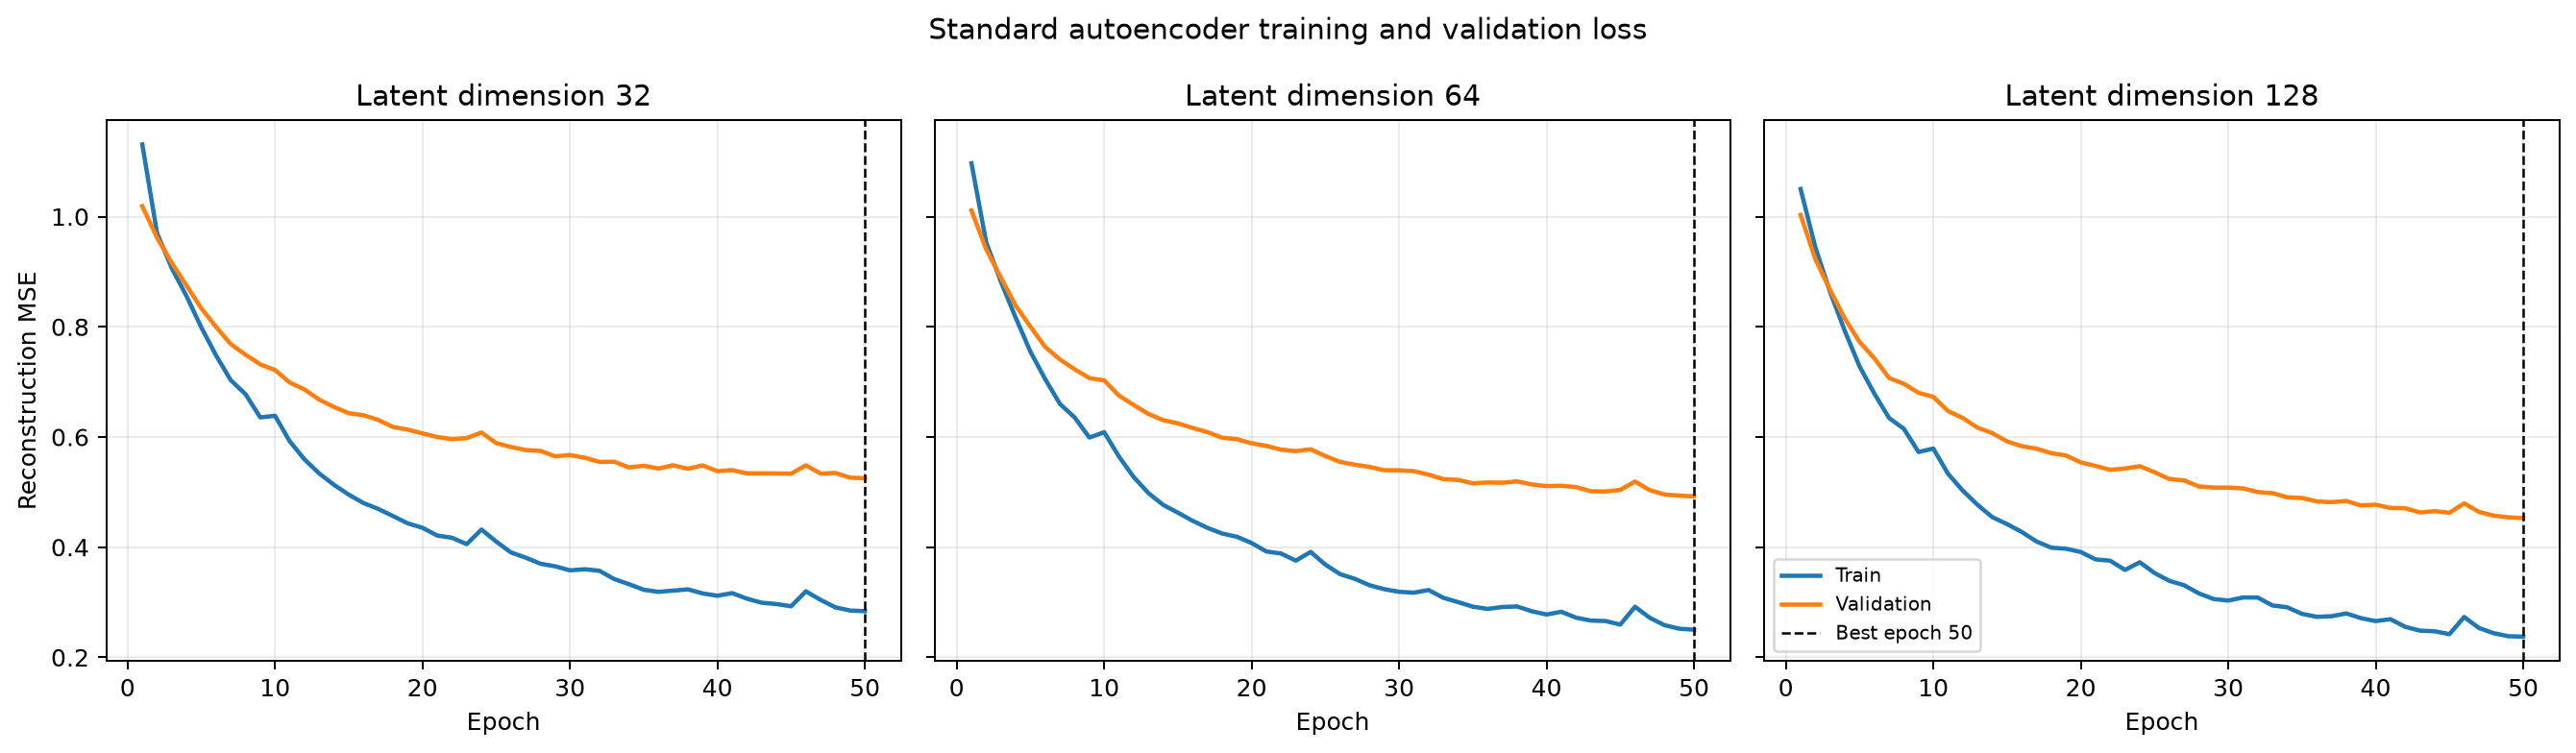
\includegraphics[width=\textwidth]{../results/figures/ae_training_curves.png}
\caption{Training and validation reconstruction MSE for the three AE bottlenecks. Dashed vertical lines mark the selected checkpoint epochs.}
\label{fig:ae-curves}
\end{figure}

Figure~\ref{fig:ae-curves} shows that all three validation curves are still decreasing at epoch 50 and all selected checkpoints occur at the maximum epoch. The experiment therefore identifies the best model within the allowed budget, but does not establish convergence. The widening train-validation gaps also show increasing fit to training data. Longer training with an unchanged validation-only protocol is a reasonable future experiment, but was not performed after observing test results.

The selected AE was repeated with seeds 7, 42, and 2026. Validation MSE values were 0.449218, 0.452771, and 0.469885, giving mean $0.457292$ and sample standard deviation $0.011050$. This modest variation indicates more stable validation behavior than the selected VAE, but three seeds cannot characterize all optimization uncertainty.

\section{Variational Autoencoder Experiments}
All VAE runs use latent dimension 64 and 175,366 trainable parameters. Table~\ref{tab:vae} reports checkpoint metrics at the validation-selected epoch. The $\beta=0.5$ model yields the best reconstruction and retains 34 active units. At $\beta=1$, only two units remain active at the final epoch; at $\beta=4$, three remain active. Both are flagged for severe collapse. The lower KL values at larger $\beta$ therefore do not indicate a better representation; they accompany reduced posterior usage.

\begin{table}[htbp]
\caption{VAE Validation Results, Latent Dimension 64 and Seed 42}
\label{tab:vae}
\centering
\small
\begin{tabular}{rrrrrrr}
\toprule
$\beta$ & Best epoch & Recon. MSE & KL/obs. & Active at best & Final active & Collapse \\
\midrule
0.5 & 50 & \metricbest{1.012741} & 0.626941 & 34 & 34 & No \\
1.0 & 30 & 1.021578 & 0.286190 & 9 & 2 & Yes \\
4.0 & 37 & 1.021564 & 0.227492 & 3 & 3 & Yes \\
\bottomrule
\end{tabular}
\end{table}

\begin{figure}[htbp]
\centering
\begin{minipage}{\textwidth}
\centering
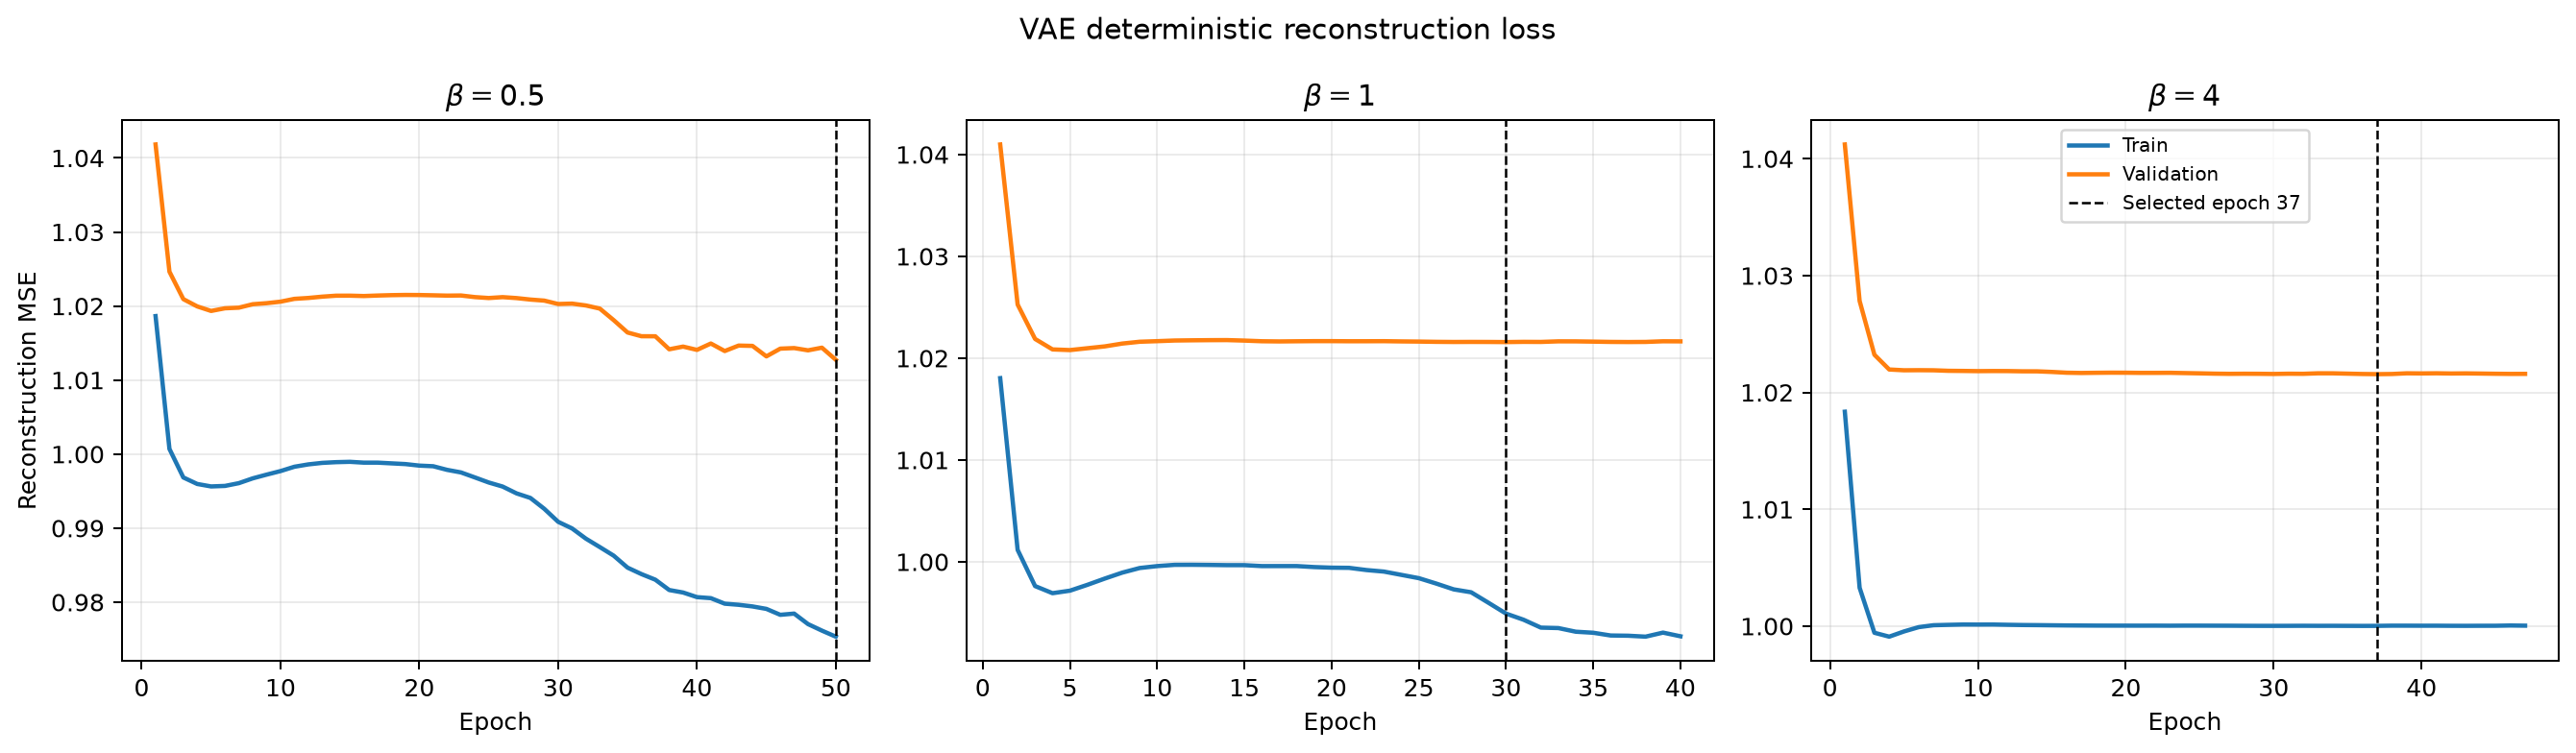
\includegraphics[width=\textwidth]{../results/figures/vae_reconstruction_curves.png}
\small (a) Deterministic reconstruction MSE.
\end{minipage}

\begin{minipage}{\textwidth}
\centering
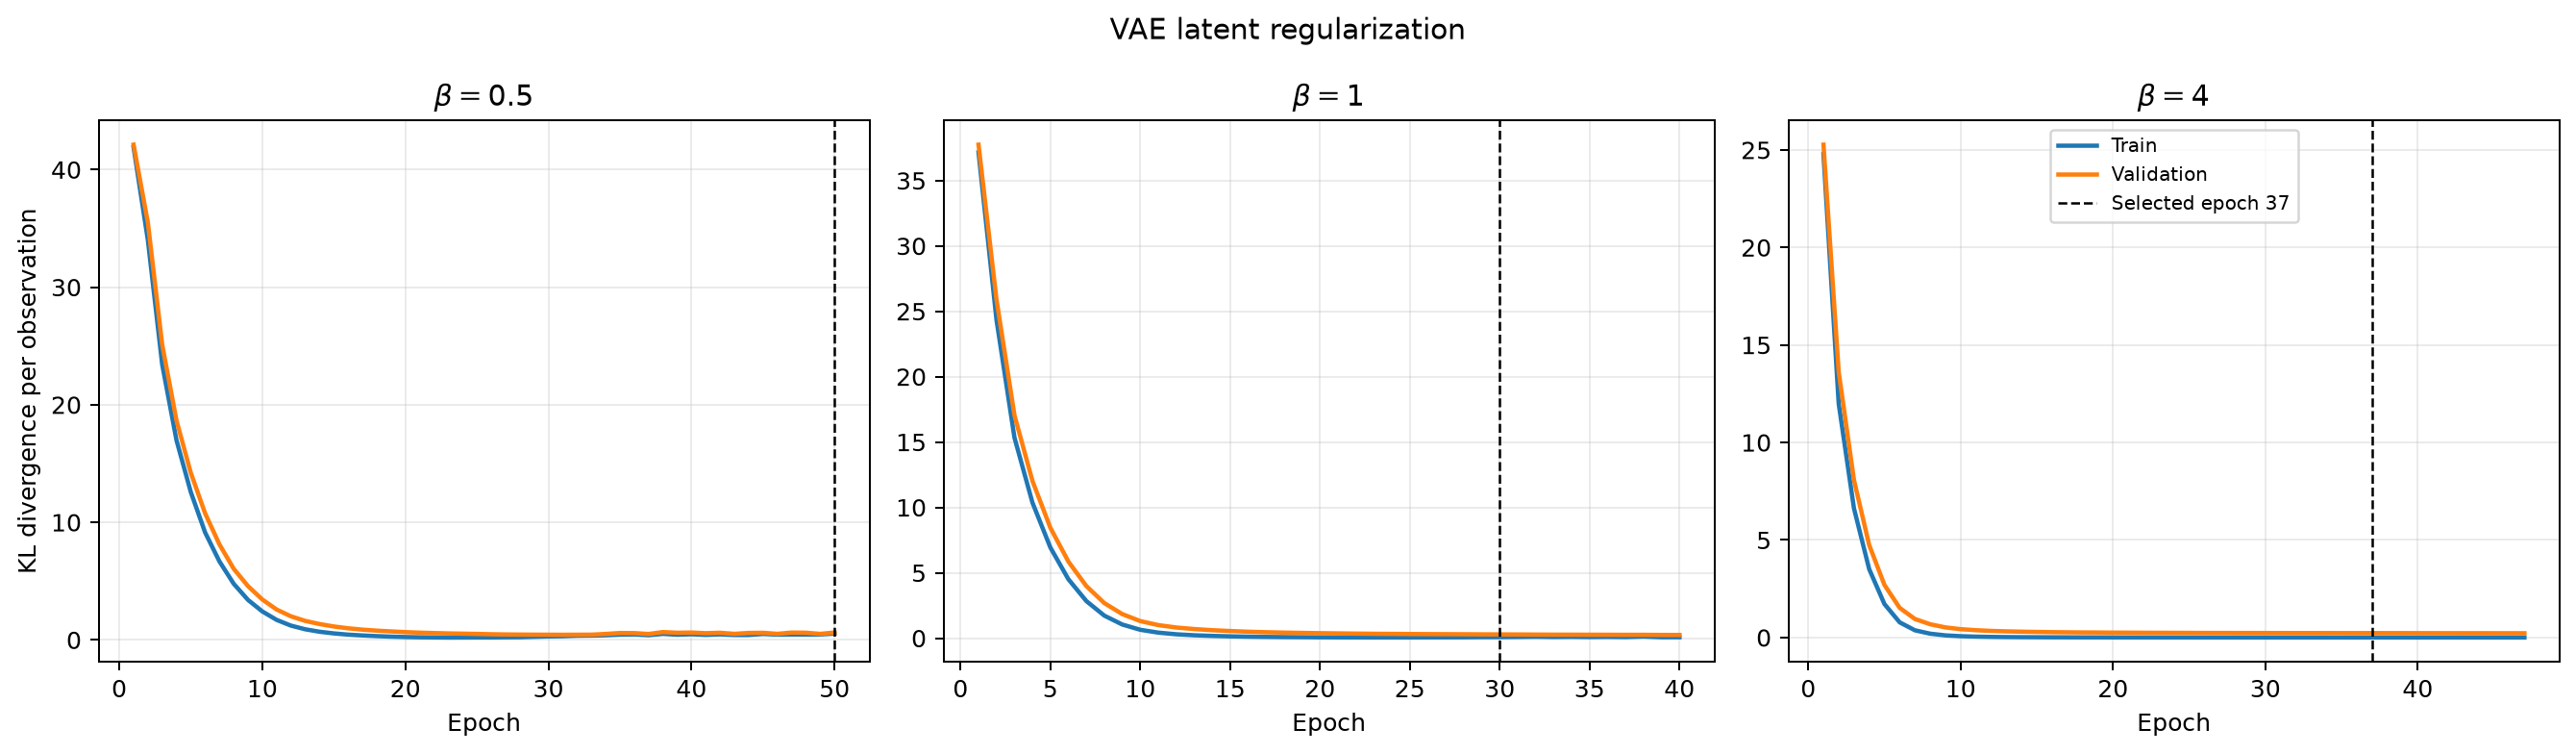
\includegraphics[width=\textwidth]{../results/figures/vae_kl_curves.png}
\small (b) Gaussian KL summed over latent dimensions per observation.
\end{minipage}
\caption{VAE validation behavior for the three target $\beta$ values. The ten-epoch warmup precedes validation-only checkpoint selection.}
\label{fig:vae-curves}
\end{figure}

The deterministic AE $q=64$ validation MSE is 0.492260, less than half the selected VAE's 1.012741. This controlled equal-latent-width comparison shows the reconstruction cost of the implemented stochastic regularization. The VAE curves in Fig.~\ref{fig:vae-curves} also end at epoch 50 for $\beta=0.5$, so its best non-collapsed run remains limited by the training budget.

\begin{figure}[htbp]
\centering
\begin{minipage}[t]{0.49\textwidth}
\centering
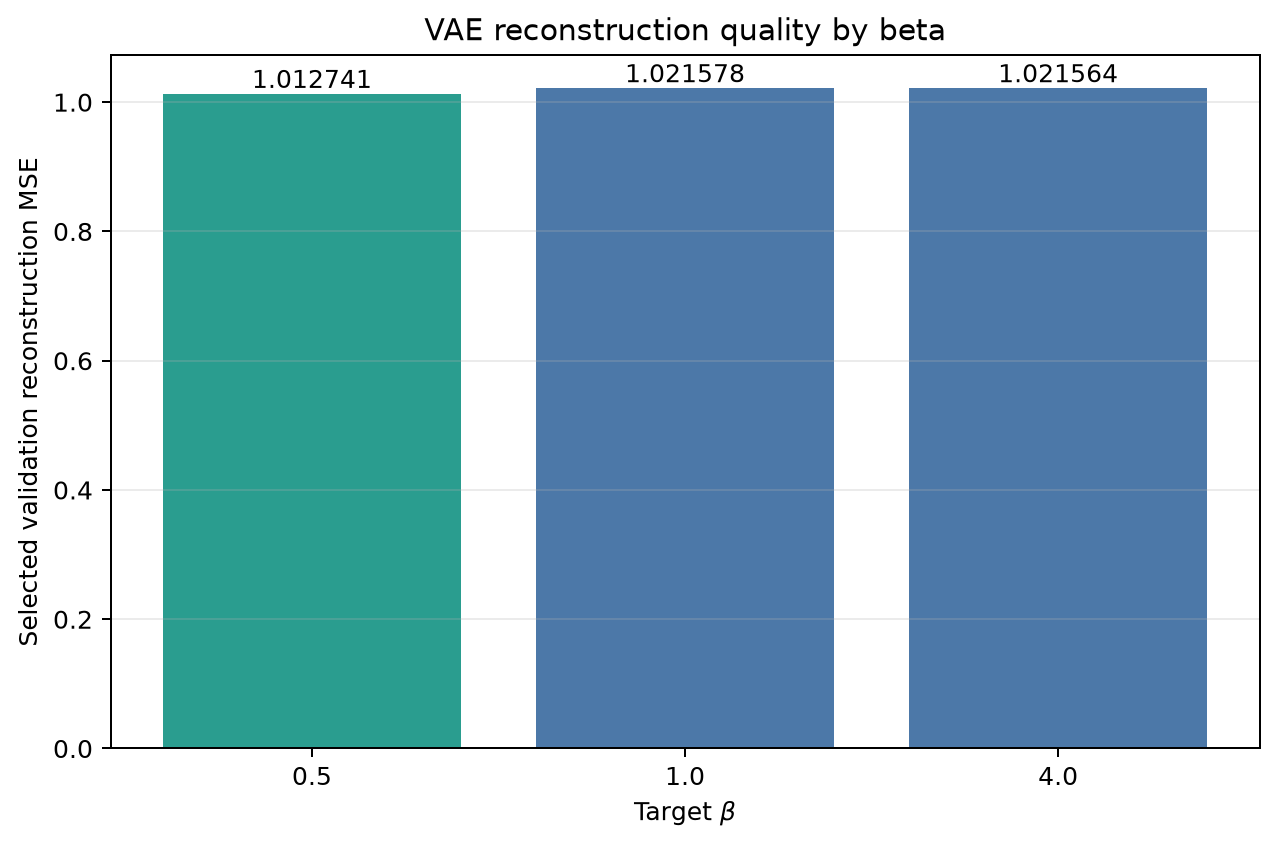
\includegraphics[width=\textwidth]{../results/figures/vae_validation_reconstruction_by_beta.png}
\small (a) Validation reconstruction by $\beta$.
\end{minipage}\hfill
\begin{minipage}[t]{0.49\textwidth}
\centering
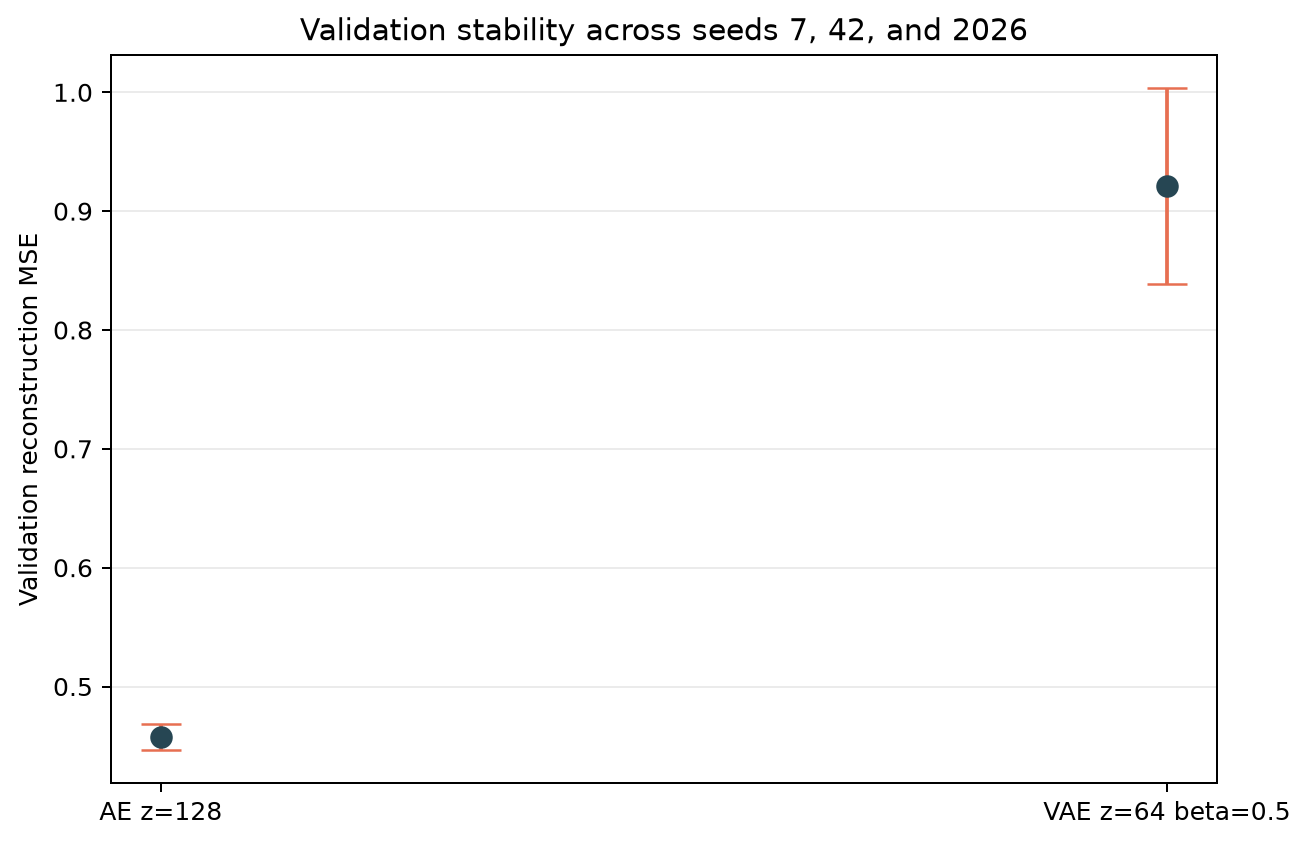
\includegraphics[width=\textwidth]{../results/figures/ae_vae_seed_stability.png}
\small (b) Three-seed stability.
\end{minipage}
\caption{VAE selection and stability evidence. Error bars in (b) summarize seeds 7, 42, and 2026.}
\label{fig:vae-selection}
\end{figure}

Across seeds 7, 42, and 2026, the selected VAE produced validation MSE values 0.853488, 1.012741, and 0.896869, with mean $0.921033$ and sample standard deviation $0.082330$. Active-unit counts at the selected checkpoints were 64, 34, and 64. The larger variability than the AE confirms sensitivity to initialization and optimization, and it prevents interpreting the seed-42 checkpoint as a complete description of VAE performance.

\section{Reconstruction Evaluation}
The frozen checkpoints were loaded without retraining. The VAE uses its posterior mean for deterministic reconstruction. Table~\ref{tab:reconstruction} shows that the AE is substantially better globally and on continuous variables. The VAE has slightly smaller one-hot MAE, 0.330044 versus 0.335283, but worse one-hot MSE and much lower correlation. This pattern is consistent with predictions concentrated near frequent values rather than case-specific recovery.

\begin{table}[htbp]
\caption{Frozen Reconstruction Results on the Fixed Test Set ($N=440$)}
\label{tab:reconstruction}
\centering
\begin{tabular}{llrrrr}
\toprule
Model & Feature group & Features & MSE & MAE & Pearson $r$ \\
\midrule
AE & All & 262 & \metricbest{0.399277} & \metricbest{0.359611} & \metricbest{0.762230} \\
AE & Continuous & 62 & 0.442426 & 0.438086 & 0.754514 \\
AE & One-hot & 200 & 0.385901 & 0.335283 & 0.764806 \\
\addlinespace
VAE & All & 262 & 0.940321 & 0.419778 & 0.091476 \\
VAE & Continuous & 62 & 1.017783 & 0.709241 & 0.075016 \\
VAE & One-hot & 200 & 0.916308 & \metricbest{0.330044} & 0.097469 \\
\bottomrule
\end{tabular}
\end{table}

\begin{figure}[htbp]
\centering
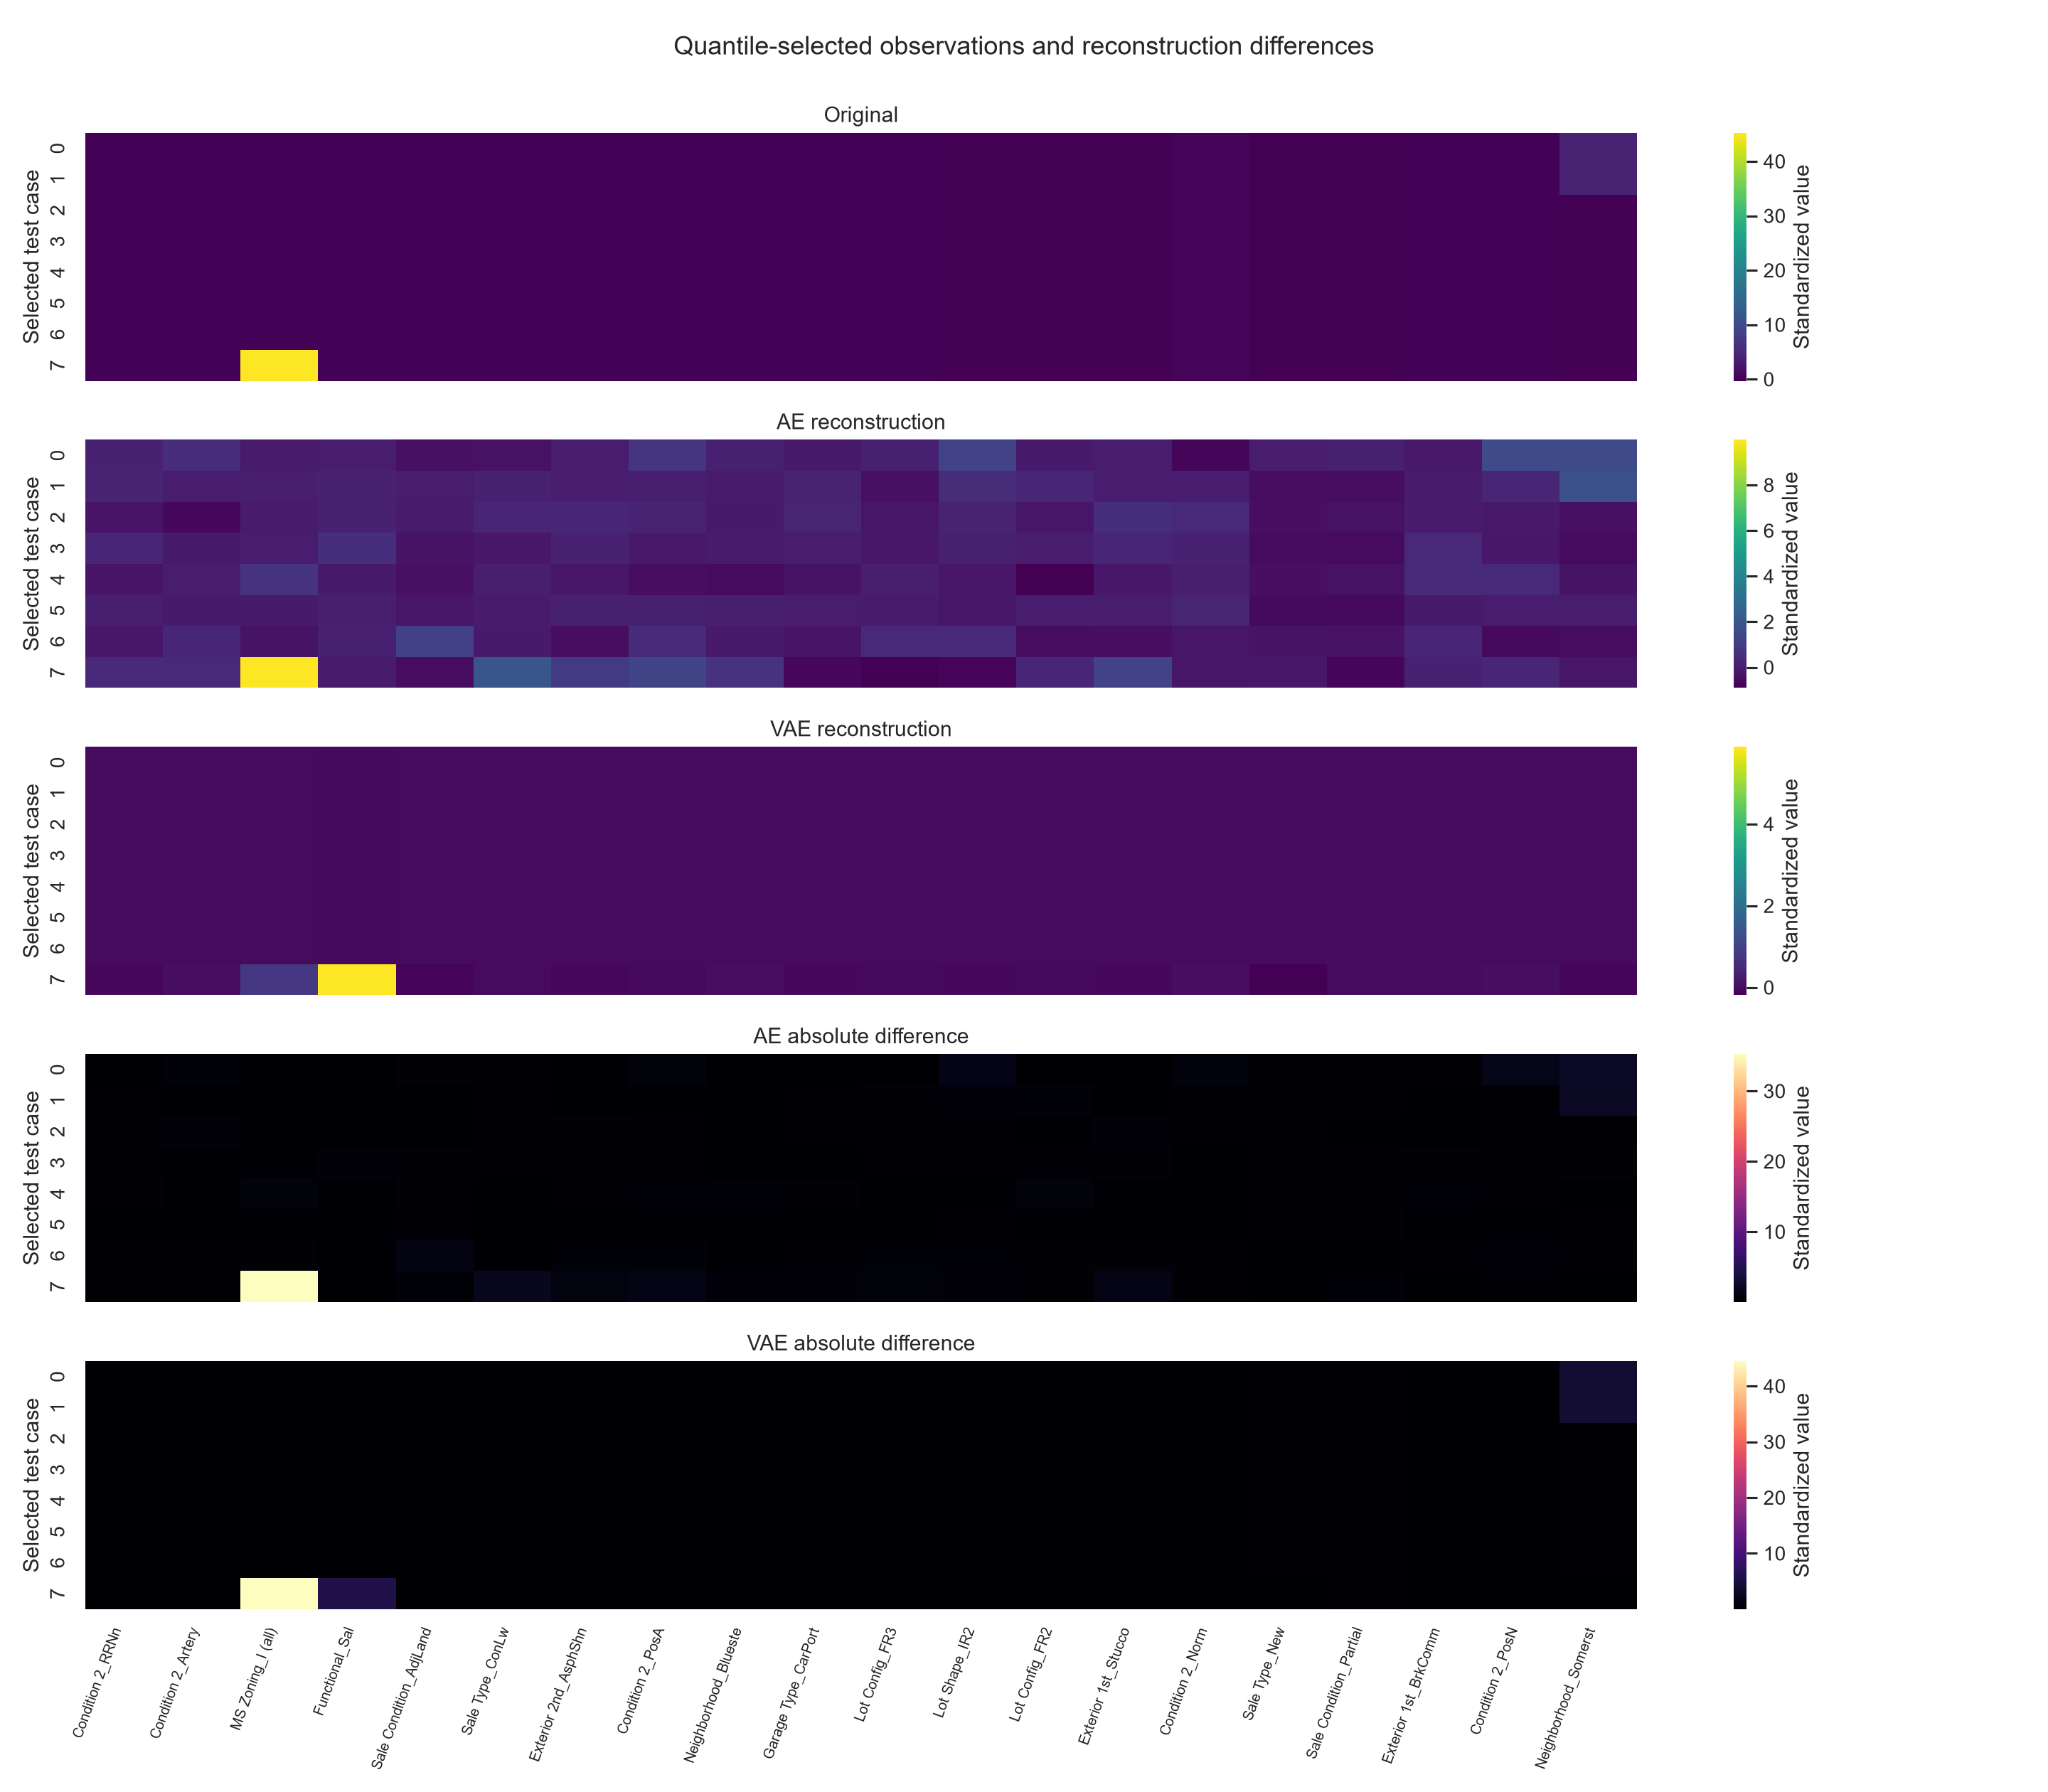
\includegraphics[width=0.92\textwidth]{../results/figures/reconstruction/reconstruction_heatmaps.png}
\caption{Original values, deterministic reconstructions, and absolute differences for eight quantile-selected test observations. Columns show the twenty features with the largest mean absolute AE error.}
\label{fig:reconstruction-heatmap}
\end{figure}

Figure~\ref{fig:reconstruction-heatmap} reveals that the largest-error case contains an extreme standardized value that both models fail to reproduce. Errors also concentrate in rare indicators and variables with unusual magnitudes. The heatmap uses different color scales by panel, so color intensity must be interpreted through each color bar rather than compared visually without calibration. Aggregate MSE is dominated by a limited number of large standardized errors, whereas MAE better describes the typical absolute deviation.

\begin{figure}[htbp]
\centering
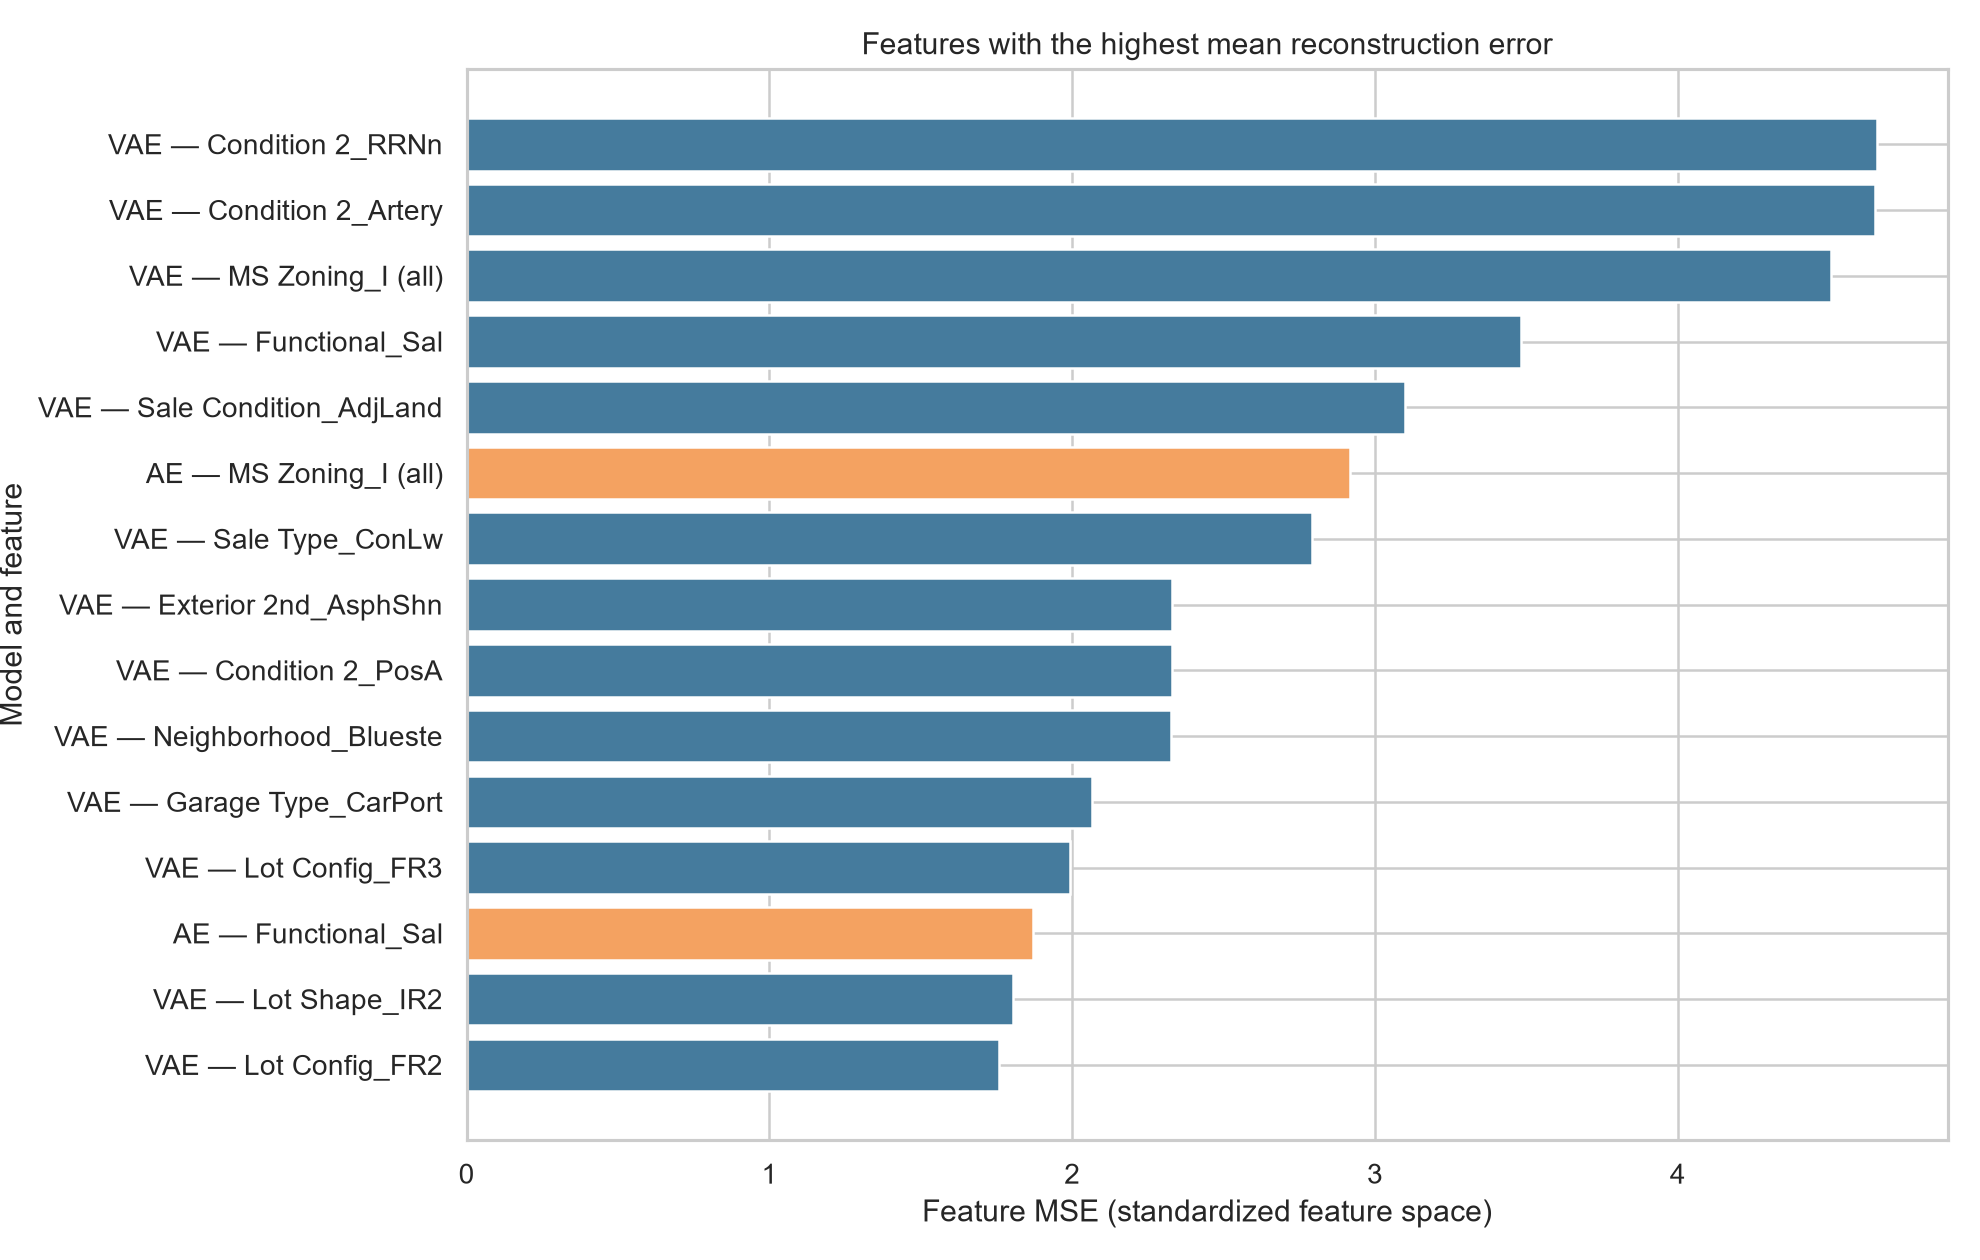
\includegraphics[width=0.82\textwidth]{../results/figures/reconstruction/highest_error_features.png}
\caption{Features with the largest mean reconstruction MSE on test. Values remain in the train-standardized transformed space.}
\label{fig:feature-errors}
\end{figure}

\section{Anomaly Detection}
The anomaly experiment retrains separate AE and VAE models only on Normal transactions using the 248-input label-free matrix. The AE and VAE checkpoints are selected on Normal validation reconstruction; the 95th-percentile thresholds are also fitted on those validation scores. The primary test comparison contains 353 Normal and 19 Abnorml transactions. Other sale conditions remain in the score artifact but are excluded from binary metrics.

\begin{table}[htbp]
\caption{Transaction-Anomaly Results on Normal versus Abnorml Test Cases}
\label{tab:anomaly}
\centering
\scriptsize
\setlength{\tabcolsep}{3.1pt}
\begin{tabular}{lrrrrrr}
\toprule
Score & ROC-AUC & PR-AUC & Precision & Recall & F1 & TN/FP/FN/TP \\
\midrule
AE MSE & \metricbest{0.6317} & 0.1330 & \metricbest{0.2308} & \metricbest{0.1579} & \metricbest{0.1875} & 343/10/16/3 \\
VAE MSE & 0.6071 & \metricbest{0.1414} & 0.1818 & 0.1053 & 0.1333 & 344/9/17/2 \\
VAE MSE + $0.5$ KL/$q$ & 0.6064 & 0.1413 & 0.1667 & 0.1053 & 0.1290 & 343/10/17/2 \\
\bottomrule
\end{tabular}

\vspace{0.4em}
\footnotesize AE ROC-AUC 95\% CI: 0.4971--0.7601; AE PR-AUC 95\% CI: 0.0656--0.3074. Intervals use 2,000 stratified bootstrap replicates.
\end{table}

\begin{figure}[htbp]
\centering
\begin{minipage}{\textwidth}
\centering
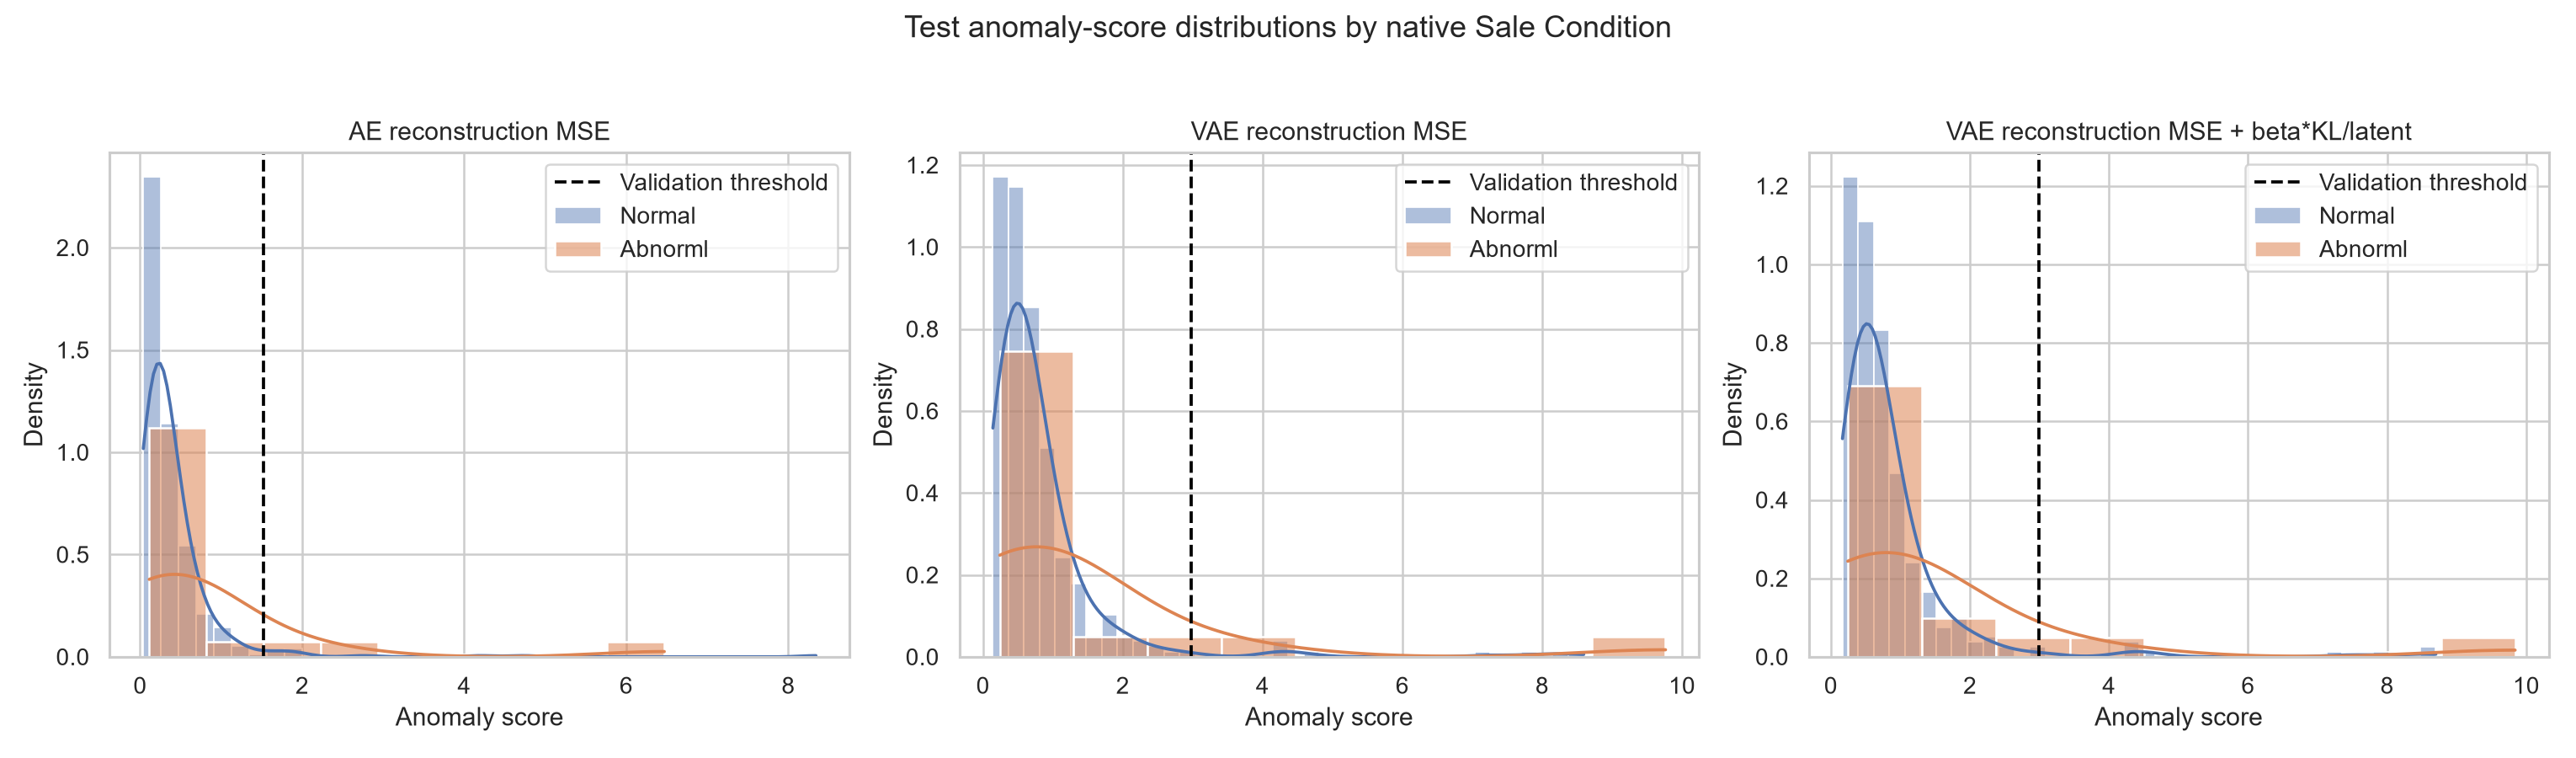
\includegraphics[width=\textwidth]{../results/figures/anomaly/anomaly_score_distributions.png}
\small (a) Score distributions by native Sale Condition.
\end{minipage}

\begin{minipage}{\textwidth}
\centering
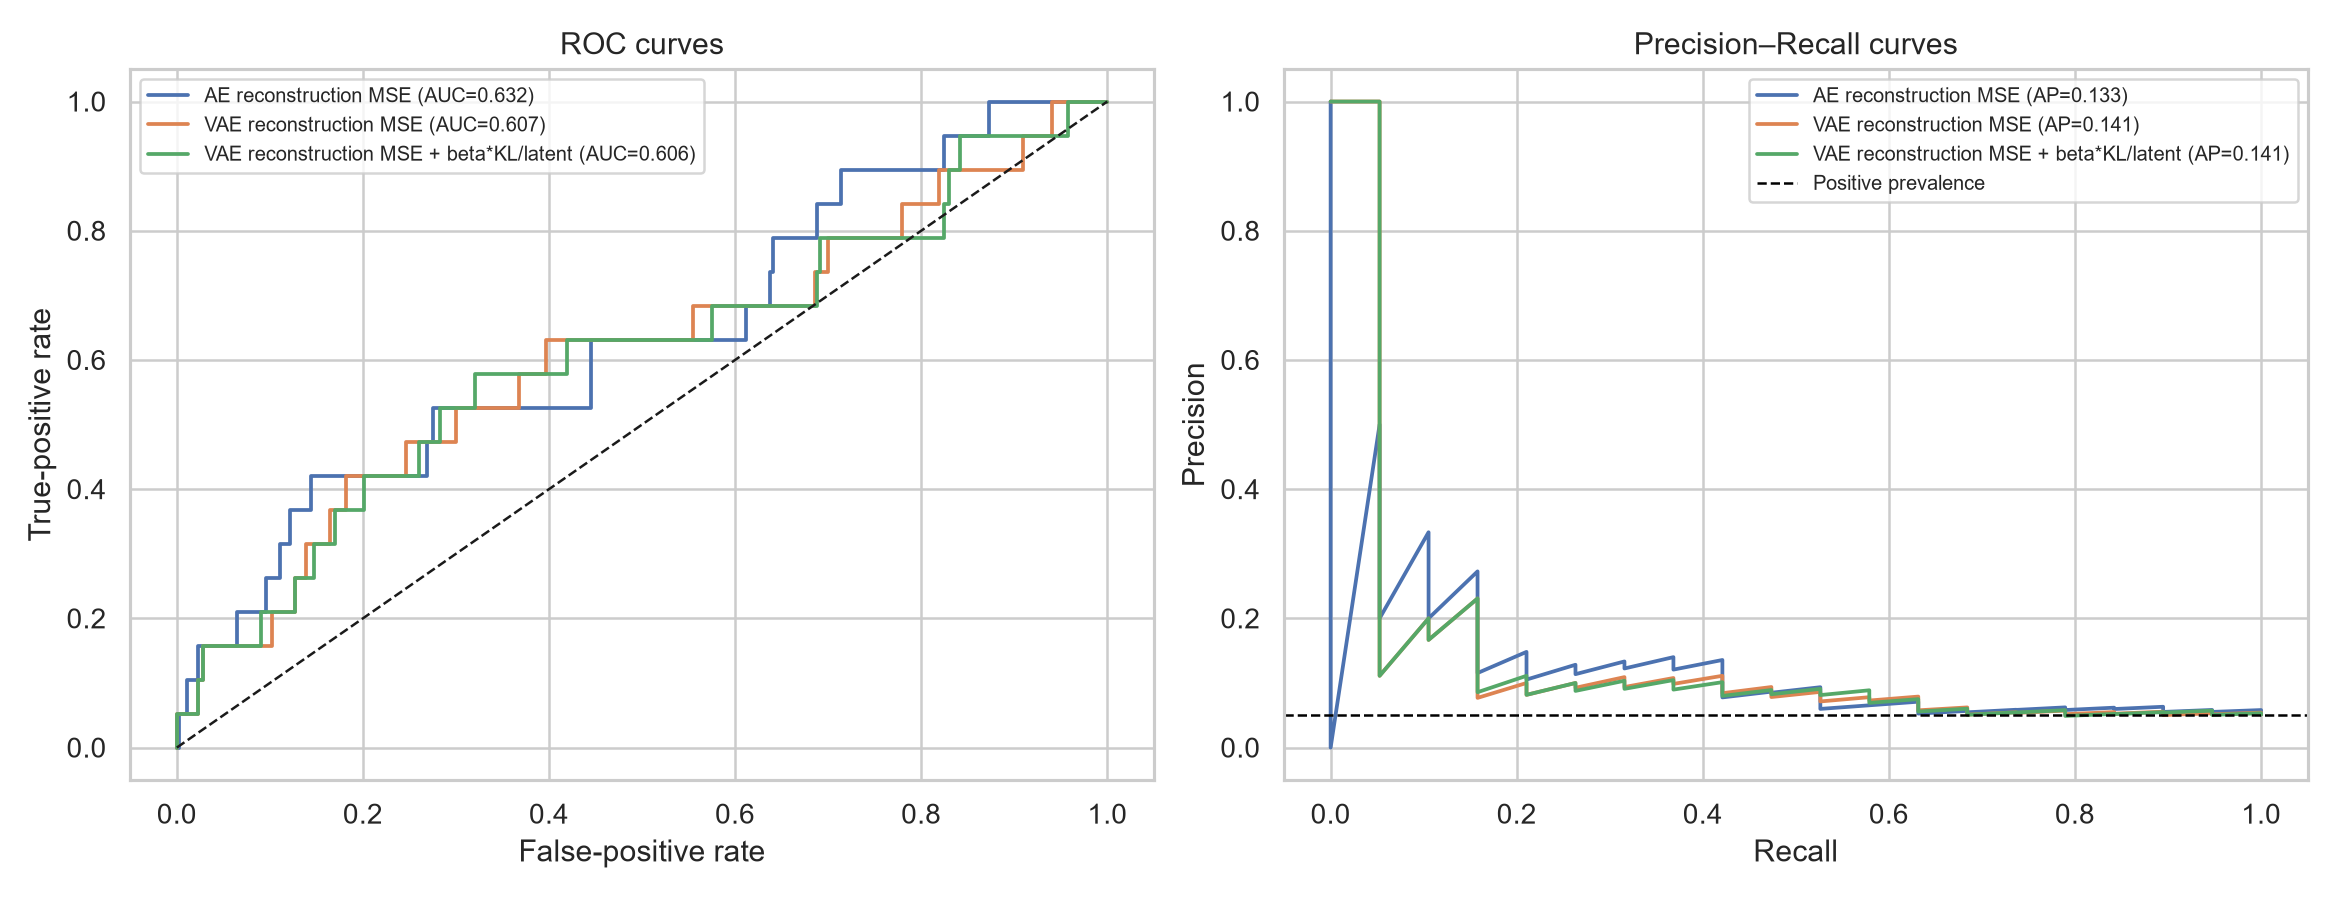
\includegraphics[width=\textwidth]{../results/figures/anomaly/anomaly_roc_precision_recall.png}
\small (b) ROC and precision-recall curves for the primary binary comparison.
\end{minipage}
\caption{Independent transaction-anomaly evaluation. Thresholds and checkpoint choices were fixed using Normal validation observations only.}
\label{fig:anomaly}
\end{figure}

Abnorml cases have higher mean reconstruction scores, but their interquartile ranges overlap strongly with Normal cases. The AE mean rises from 0.4058 to 0.8830, and the VAE reconstruction mean rises from 0.8096 to 1.4584. The AE obtains the highest ROC-AUC, recall, and F1; VAE MSE has a marginally larger PR-AUC point estimate. Adding KL does not improve discrimination. The wide intervals and the AE ROC-AUC interval crossing 0.5 prevent strong claims of reliable detection.

Most importantly, Abnorml is a sale-condition label. It may reflect transaction circumstances rather than unusual building structure. With only 19 positives, each detected or missed case changes threshold metrics substantially. The experiment therefore measures ranking of an imbalanced transaction label, not a validated structural-anomaly system.

\section{Latent Space Analysis}
Figure~\ref{fig:tsne-price} shows a clear monotonic price gradient for the supervised MLP. AE $q=64$ also displays a price progression despite never receiving SalePrice, plausibly because size, quality, age, and location jointly support reconstruction and correlate with price. AE $q=128$ is less compact in two dimensions. The VAE forms a dense concentration and branches with weaker price organization.

\begin{figure}[htbp]
\centering
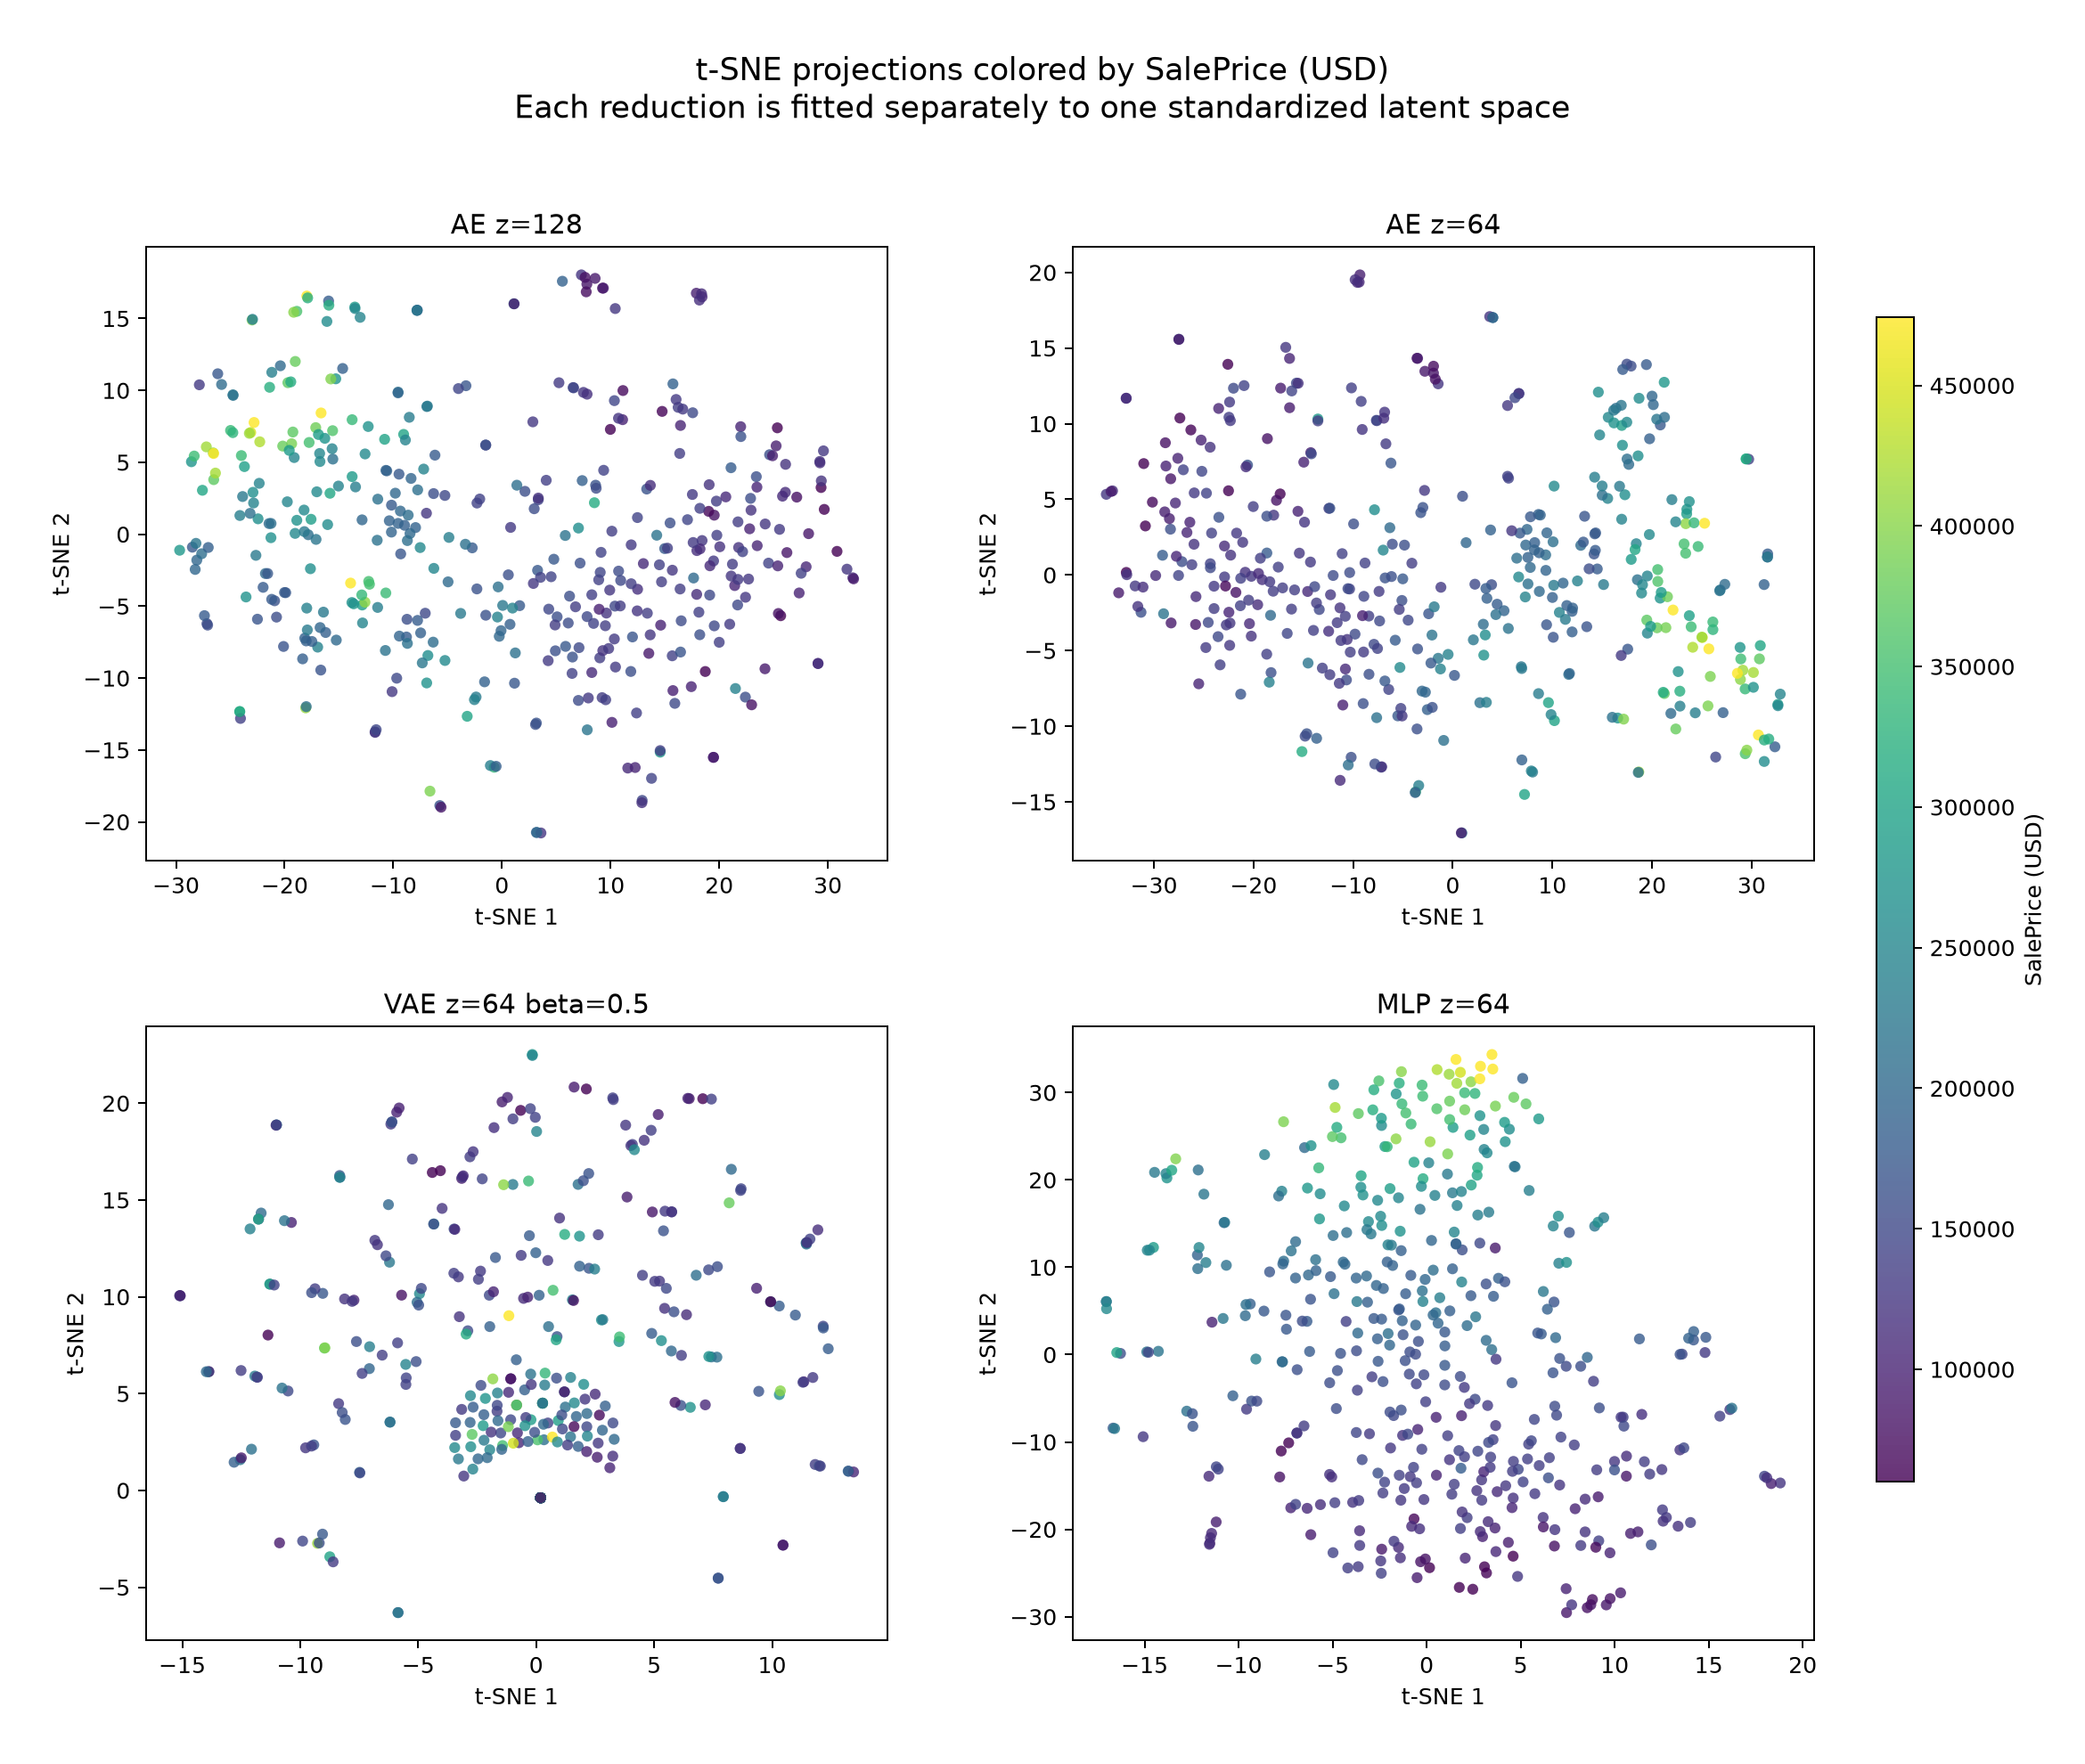
\includegraphics[width=0.92\textwidth]{../results/figures/latent/tsne_saleprice.png}
\caption{Separate t-SNE projections colored by SalePrice. Each reducer is fitted independently, so axes, rotations, scale, and distances cannot be compared directly across panels.}
\label{fig:tsne-price}
\end{figure}

\begin{figure}[htbp]
\centering
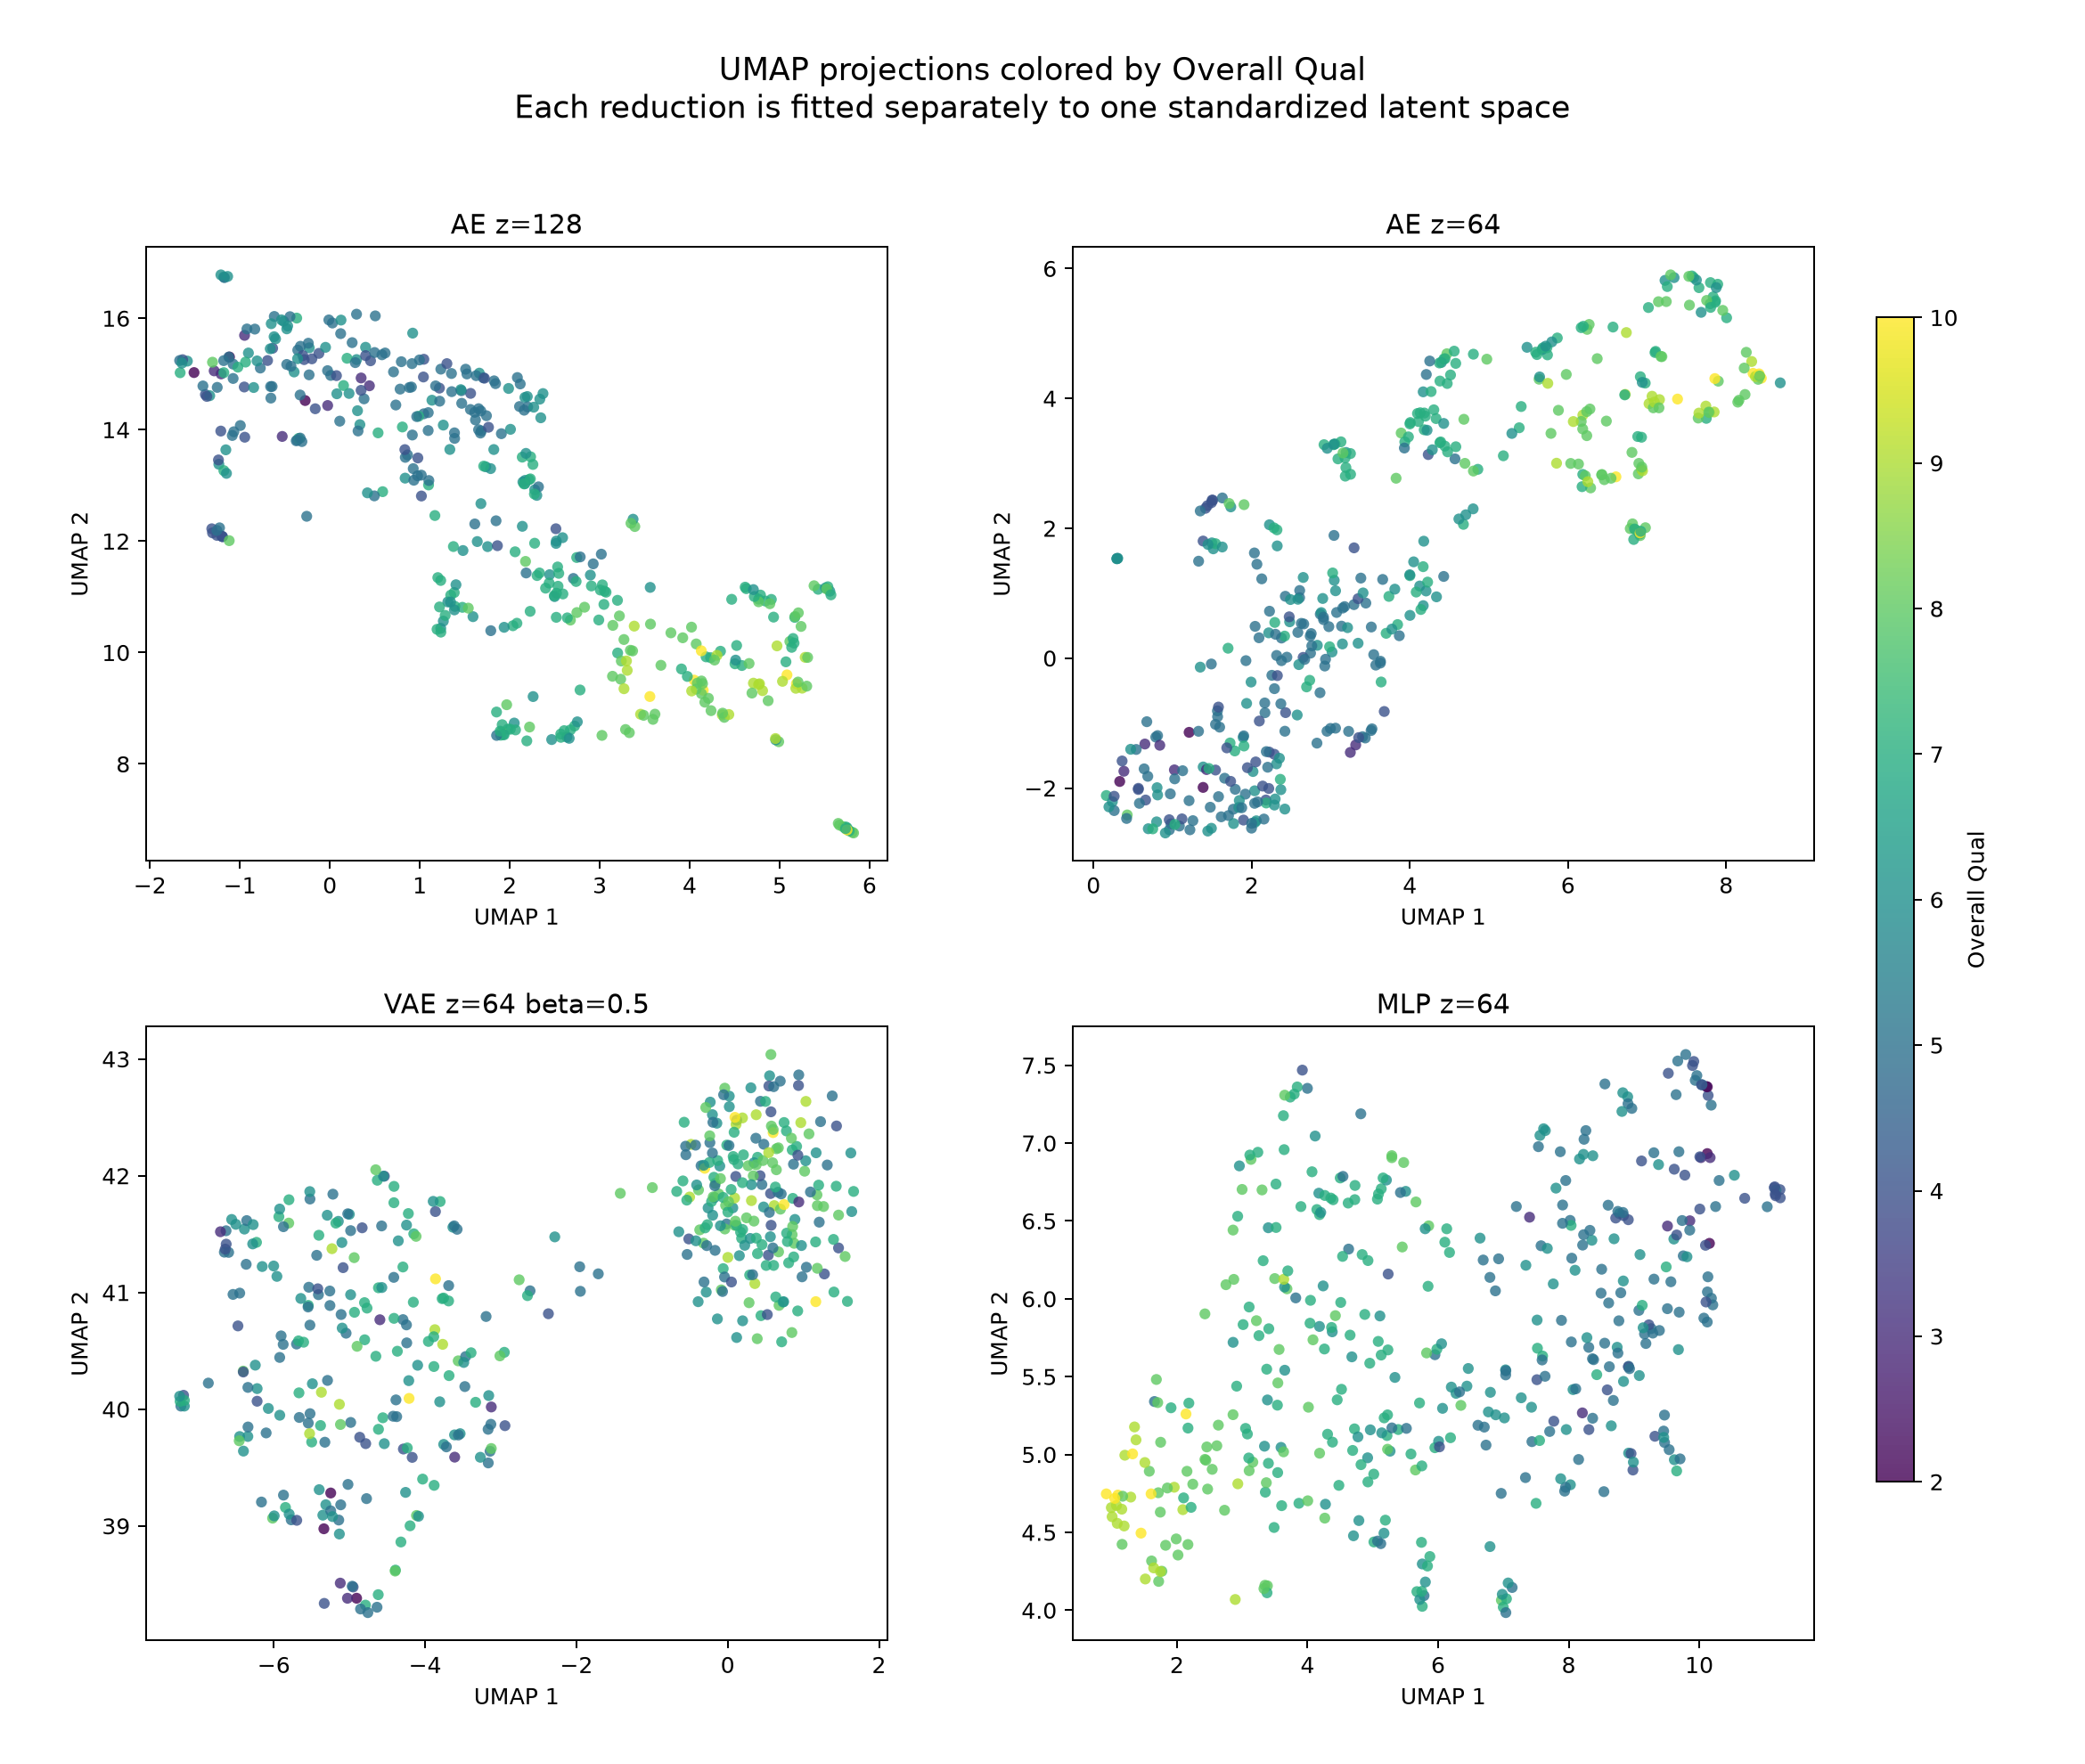
\includegraphics[width=0.92\textwidth]{../results/figures/latent/umap_overall_quality.png}
\caption{Separate UMAP projections colored by Overall Quality. Visible gradients do not imply discrete clusters; original-space Silhouette scores remain near zero or negative.}
\label{fig:umap-quality}
\end{figure}

\begin{figure}[htbp]
\centering
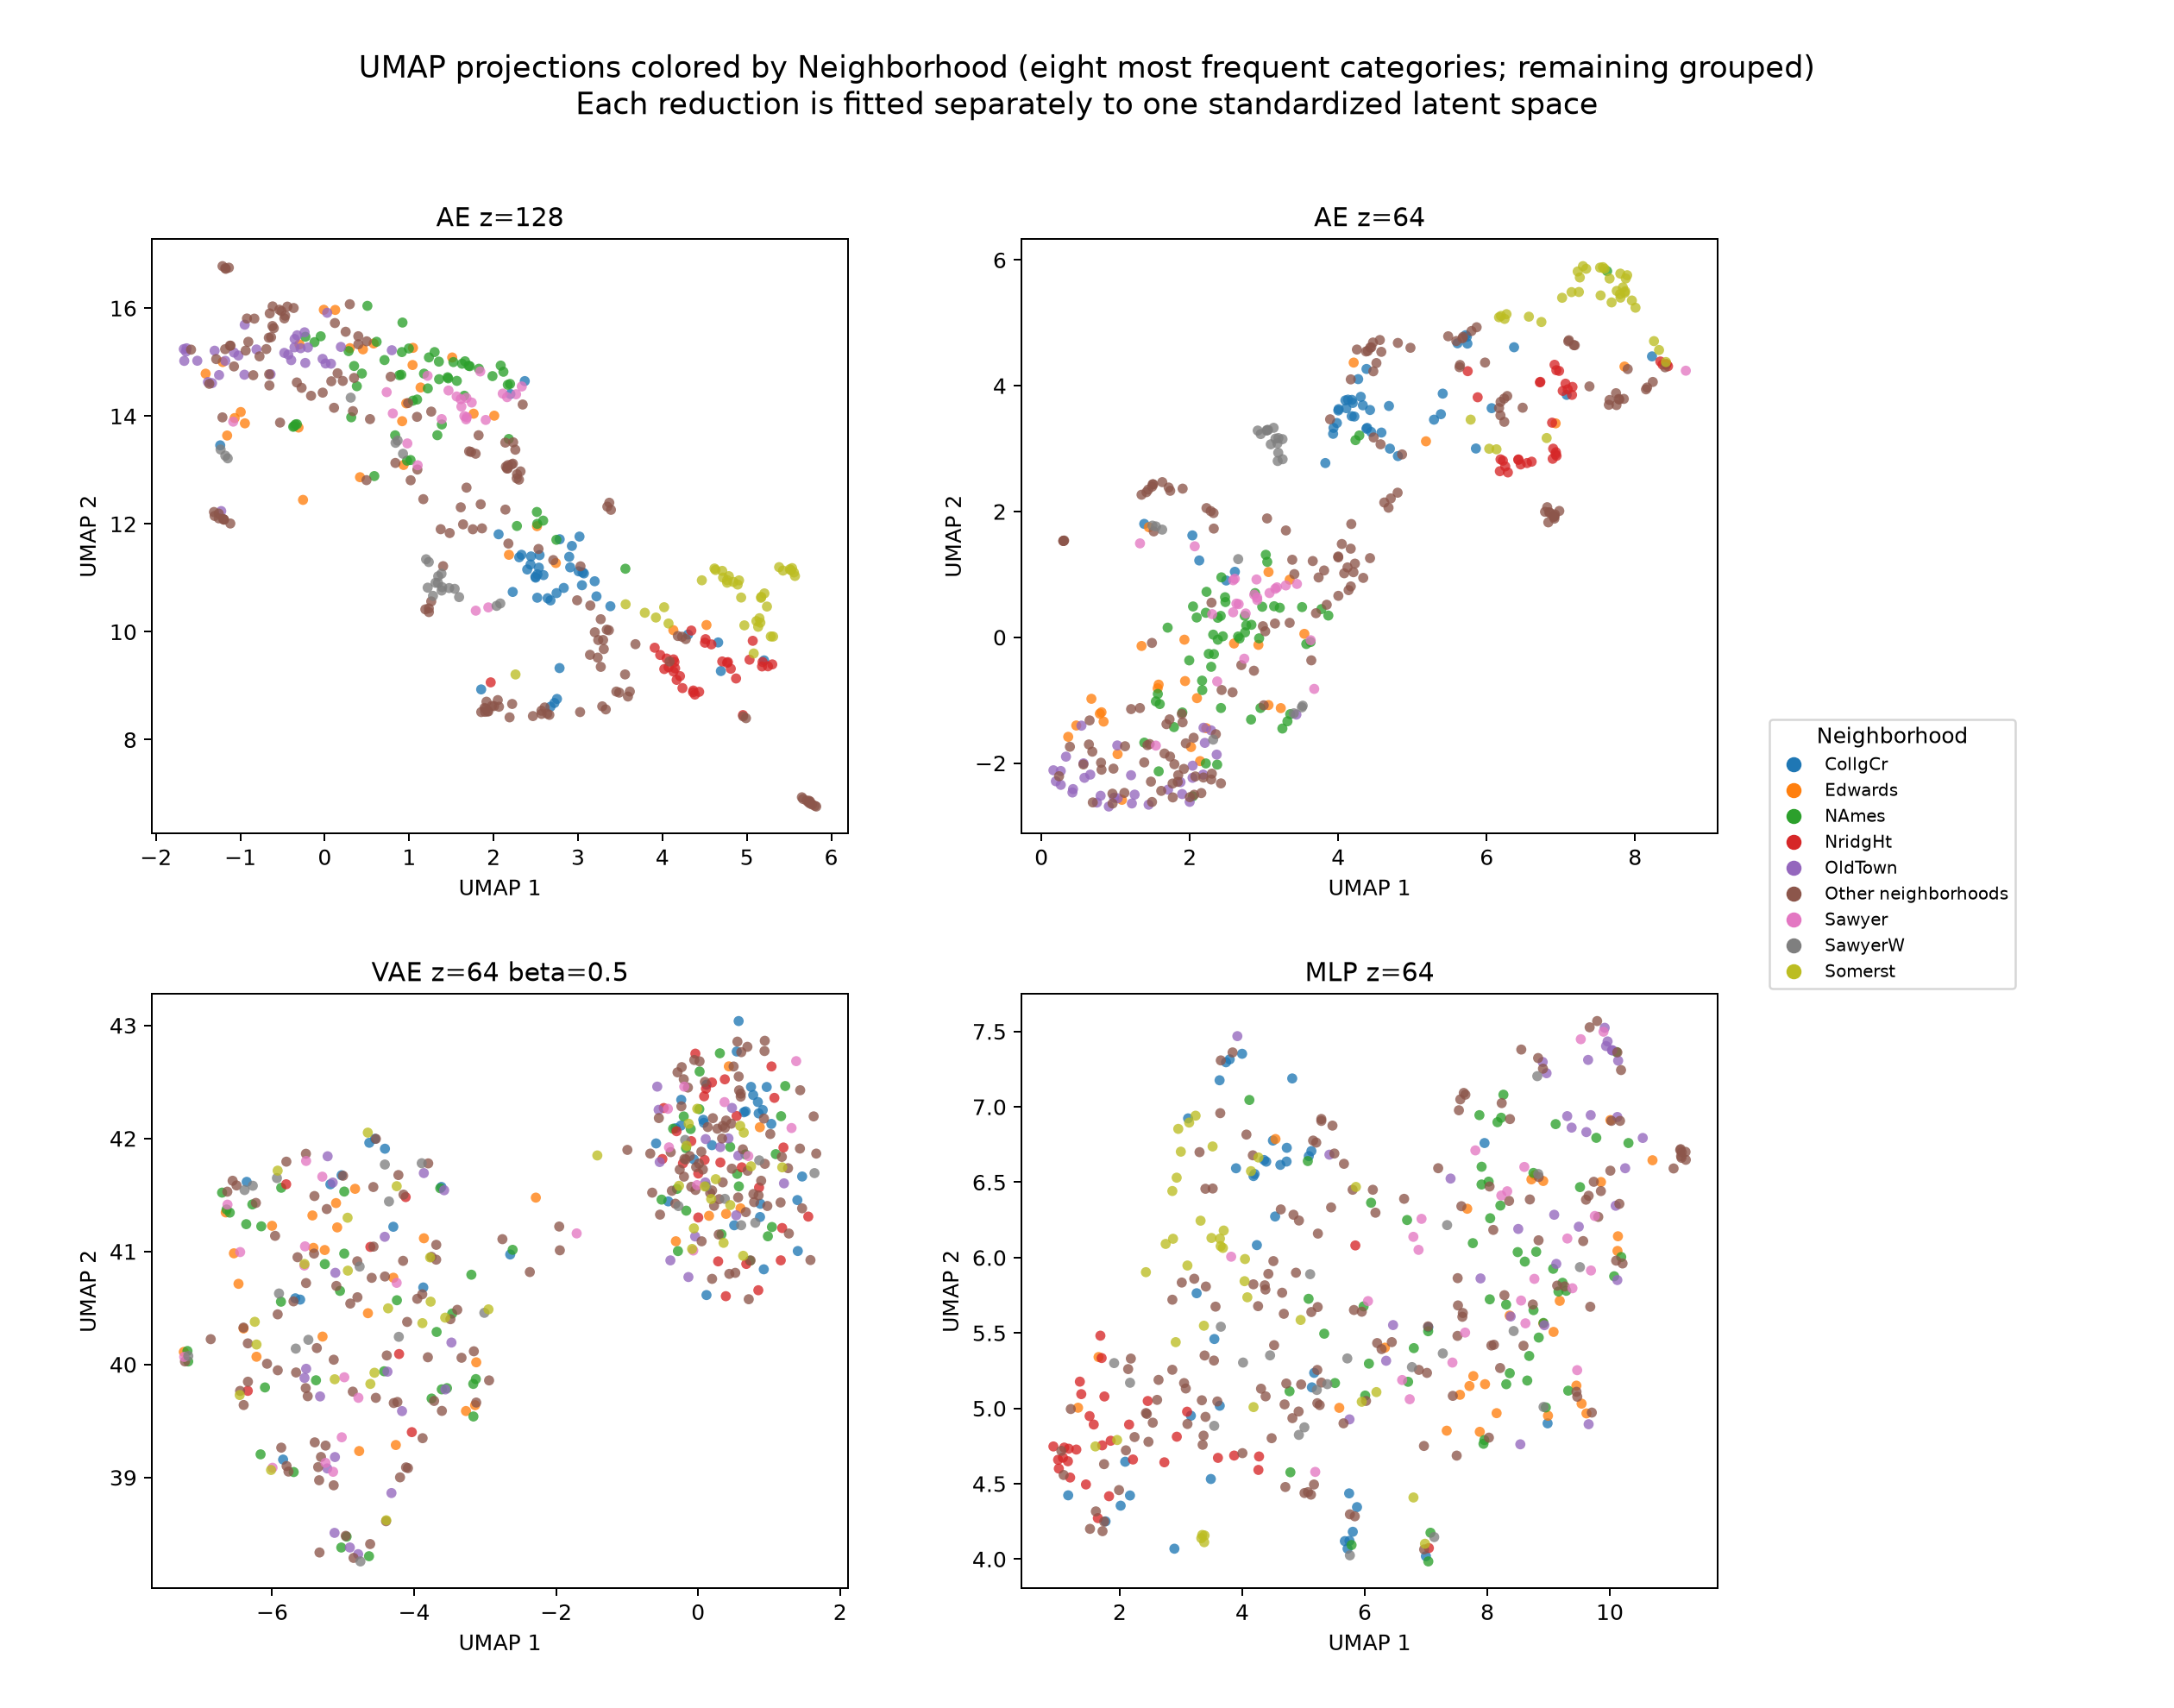
\includegraphics[width=0.92\textwidth]{../results/figures/latent/umap_neighborhood.png}
\caption{Separate UMAP projections colored by Neighborhood. The eight most frequent categories are shown individually and the remaining categories are grouped for visualization.}
\label{fig:umap-neighborhood}
\end{figure}

\begin{table}[htbp]
\caption{Original-Space Silhouette and Projection Trustworthiness}
\label{tab:latent}
\centering
\small
\begin{tabular}{lrrrrr}
\toprule
Representation & Quality & Neighborhood & Normal/Abnorml & t-SNE trust. & UMAP trust. \\
\midrule
AE $q=128$ & -0.0465 & -0.0166 & 0.1775 & 0.8395 & 0.8130 \\
AE $q=64$ & -0.0360 & -0.0222 & 0.1610 & \metricbest{0.8591} & \metricbest{0.8367} \\
VAE $q=64$, $\beta=0.5$ & -0.3836 & -0.4668 & \metricbest{0.5166} & 0.5897 & 0.6178 \\
MLP $q=64$ & \metricbest{-0.0123} & -0.1380 & 0.2466 & 0.8306 & 0.8128 \\
\bottomrule
\end{tabular}
\end{table}

Table~\ref{tab:latent} qualifies the visual interpretation. Overall Quality scores are near zero for AE and MLP and strongly negative for VAE, so color gradients should not be described as discrete clusters. Neighborhood is also mixed; both AEs are close to zero, while MLP and VAE are more negative. The VAE has the largest Normal/Abnorml Silhouette, 0.5166, but this does not contradict its modest anomaly ROC-AUC: Silhouette measures supplied-label geometry, whereas ROC-AUC measures score ranking. It also uses only 19 positive cases.

AE $q=64$ has the highest t-SNE and UMAP trustworthiness. The VAE values, 0.5897 and 0.6178, are much lower, indicating that its two-dimensional panels preserve local neighborhoods less faithfully. Every reduction was repeated with maximum absolute coordinate difference zero under the fixed software environment. Exact repeatability does not remove sensitivity to the chosen hyperparameters or justify cross-panel distance comparisons.

\section{Comparison with Supervised Learning}
The Workshop 2 MLP and Workshop 4 encoders answer different questions. The MLP's 64-dimensional activation is optimized for standardized log-price prediction and therefore organizes price and related quality information clearly. The AEs optimize broad input reconstruction and preserve more Neighborhood association and slightly higher projection trustworthiness. The VAE regularization produces a less case-specific representation under the implemented objective.

No reconstruction metric is reported for the MLP because it has no decoder, and no dollar-scale price metric is reported for AE/VAE because they are not price predictors. The comparison is therefore representational rather than a common predictive leaderboard. The most defensible conclusion is that supervision concentrates the MLP representation around the target, while deterministic reconstruction retains broader local input structure.

\section{Discussion and Limitations}
The standard AE is the strongest evaluated reconstruction model. Its validation and test MSE are both substantially lower than those of the VAE, and its correlations show meaningful case-specific recovery. However, every AE configuration is still improving at epoch 50, so the selected $q=128$ checkpoint is the best within a capped budget rather than a demonstrably converged optimum. Increasing $q$ also increases parameter count, preventing a pure latent-dimension causal claim.

The VAE study demonstrates a practical reconstruction-regularization trade-off. Larger $\beta$ values reduce KL but lead to two or three active final units, which is consistent with posterior collapse rather than useful compression. The $\beta=0.5$ model avoids the severe-collapse rule yet varies substantially across seeds. Moreover, the normalized KL objective is not an exact ELBO, so its numerical values should not be compared directly with likelihood-based VAE studies.

Mixed tabular reconstruction has intrinsic limitations. Continuous and one-hot features share an MSE objective after standardization, and a linear decoder can output invalid intermediate categorical values. Rare categories and extreme standardized observations can dominate squared error. Feature-wise reconstruction quality does not establish semantic usefulness, causality, or generative realism.

The anomaly task is particularly constrained. Sale Condition is only a proxy, the positive test class contains 19 observations, confidence intervals are wide, and a fixed 95th-percentile threshold prioritizes protocol clarity over F1 optimization. Reconstruction models may assign low error to unusual transactions or high error to rare but legitimate combinations. Accordingly, anomaly results should remain exploratory.

Finally, all models use one fixed data split. Seed repetitions measure optimization variability, not sampling variability across partitions. Latent labels are used only after training, but post-hoc interpretation can still encourage narrative overfitting. t-SNE and UMAP distort geometry, while Silhouette values depend on supplied groups and per-model standardization. The now-observed test set must not support further model or hyperparameter selection.

\subsection{Reproducibility}
Checkpoints include architecture and preprocessing metadata, and final analyses record SHA-256 hashes for the split and selected models. Reloaded checkpoints reproduce deterministic outputs exactly. AE/VAE, MLP, t-SNE, and UMAP representations use the same ordered 440 test indices. The reducers use seed 42 and reproduce coordinates within $10^{-6}$. The final academic notebook loads saved CSV, JSON, NPZ, checkpoints, and figures without training; all fifteen code cells execute successfully, with 25 embedded PNG outputs and no error outputs.

\section{Conclusions}
A leakage-aware deterministic autoencoder learned the most accurate reconstruction of the evaluated Ames Housing representations. Increasing the latent dimension from 32 to 128 reduced validation MSE to 0.452771, and the frozen selected model reached test MSE 0.399277, MAE 0.359611, and Pearson correlation 0.762230. The curves were still improving at the 50-epoch limit, so these values describe the completed experiment rather than a converged performance ceiling.

The selected $\beta=0.5$ VAE retained more latent activity than $\beta=1$ and $\beta=4$, but reconstructed less faithfully and was less stable across seeds. The anomaly protocol produced only modest discrimination, with best ROC-AUC 0.6317 and low recall on 19 Abnorml transactions. In the latent comparison, the supervised MLP most clearly reflected SalePrice, the AEs better preserved local projection neighborhoods, and no representation dominated every descriptive criterion. The central result is therefore objective-dependent: reconstruction, anomaly ranking, and supervised target organization reveal different aspects of the same housing data.

Future work should allocate a new validation protocol before extending training, investigate loss functions that distinguish continuous from categorical variables, quantify stability over multiple data splits, and evaluate anomaly labels with clearer domain meaning. Any further model selection must avoid reusing the already observed test outcomes.

\bibliographystyle{unsrt}
\bibliography{references}

\end{document}
